\chapter{Additional content}


\begin{figure}[h]
  \caption{Front page of the paper form used by EMEL during vehicle maintenance. Operators use this section to record identified malfunctions.}
  \centering
  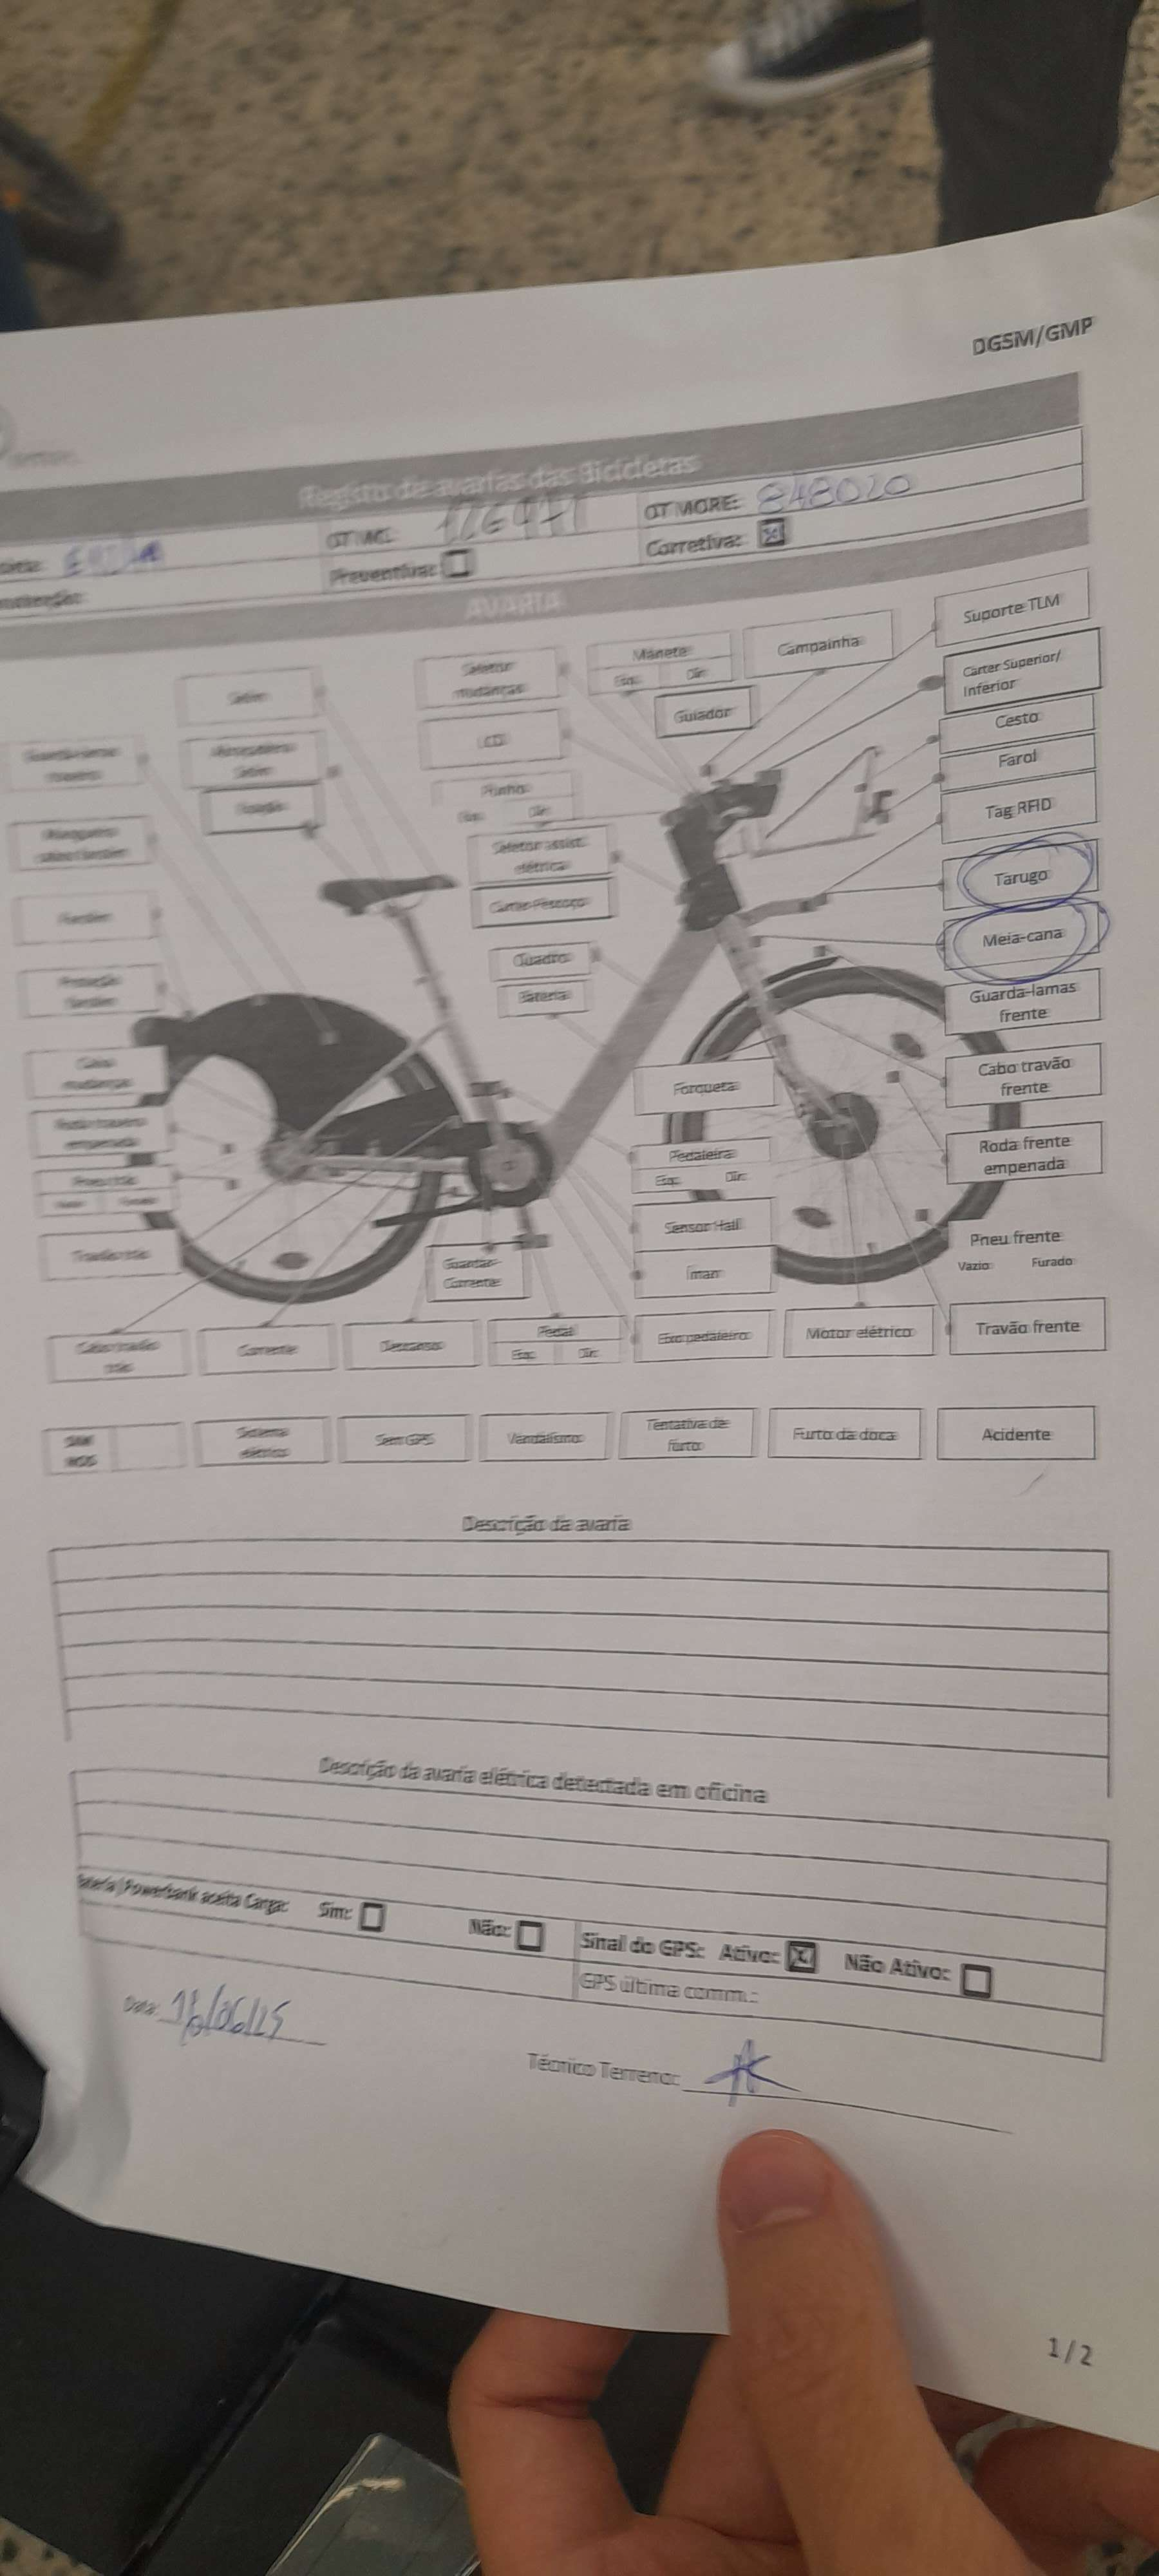
\includegraphics[width=0.50\textwidth]{figs/chapter2/emel_front}
  \label{fig:emel_front}
\end{figure}

\begin{figure}[h]
  \caption{Back page of the paper form used by EMEL during vehicle maintenance. Mechanics use this section to document the parts replaced during the repair process.}
  \centering
  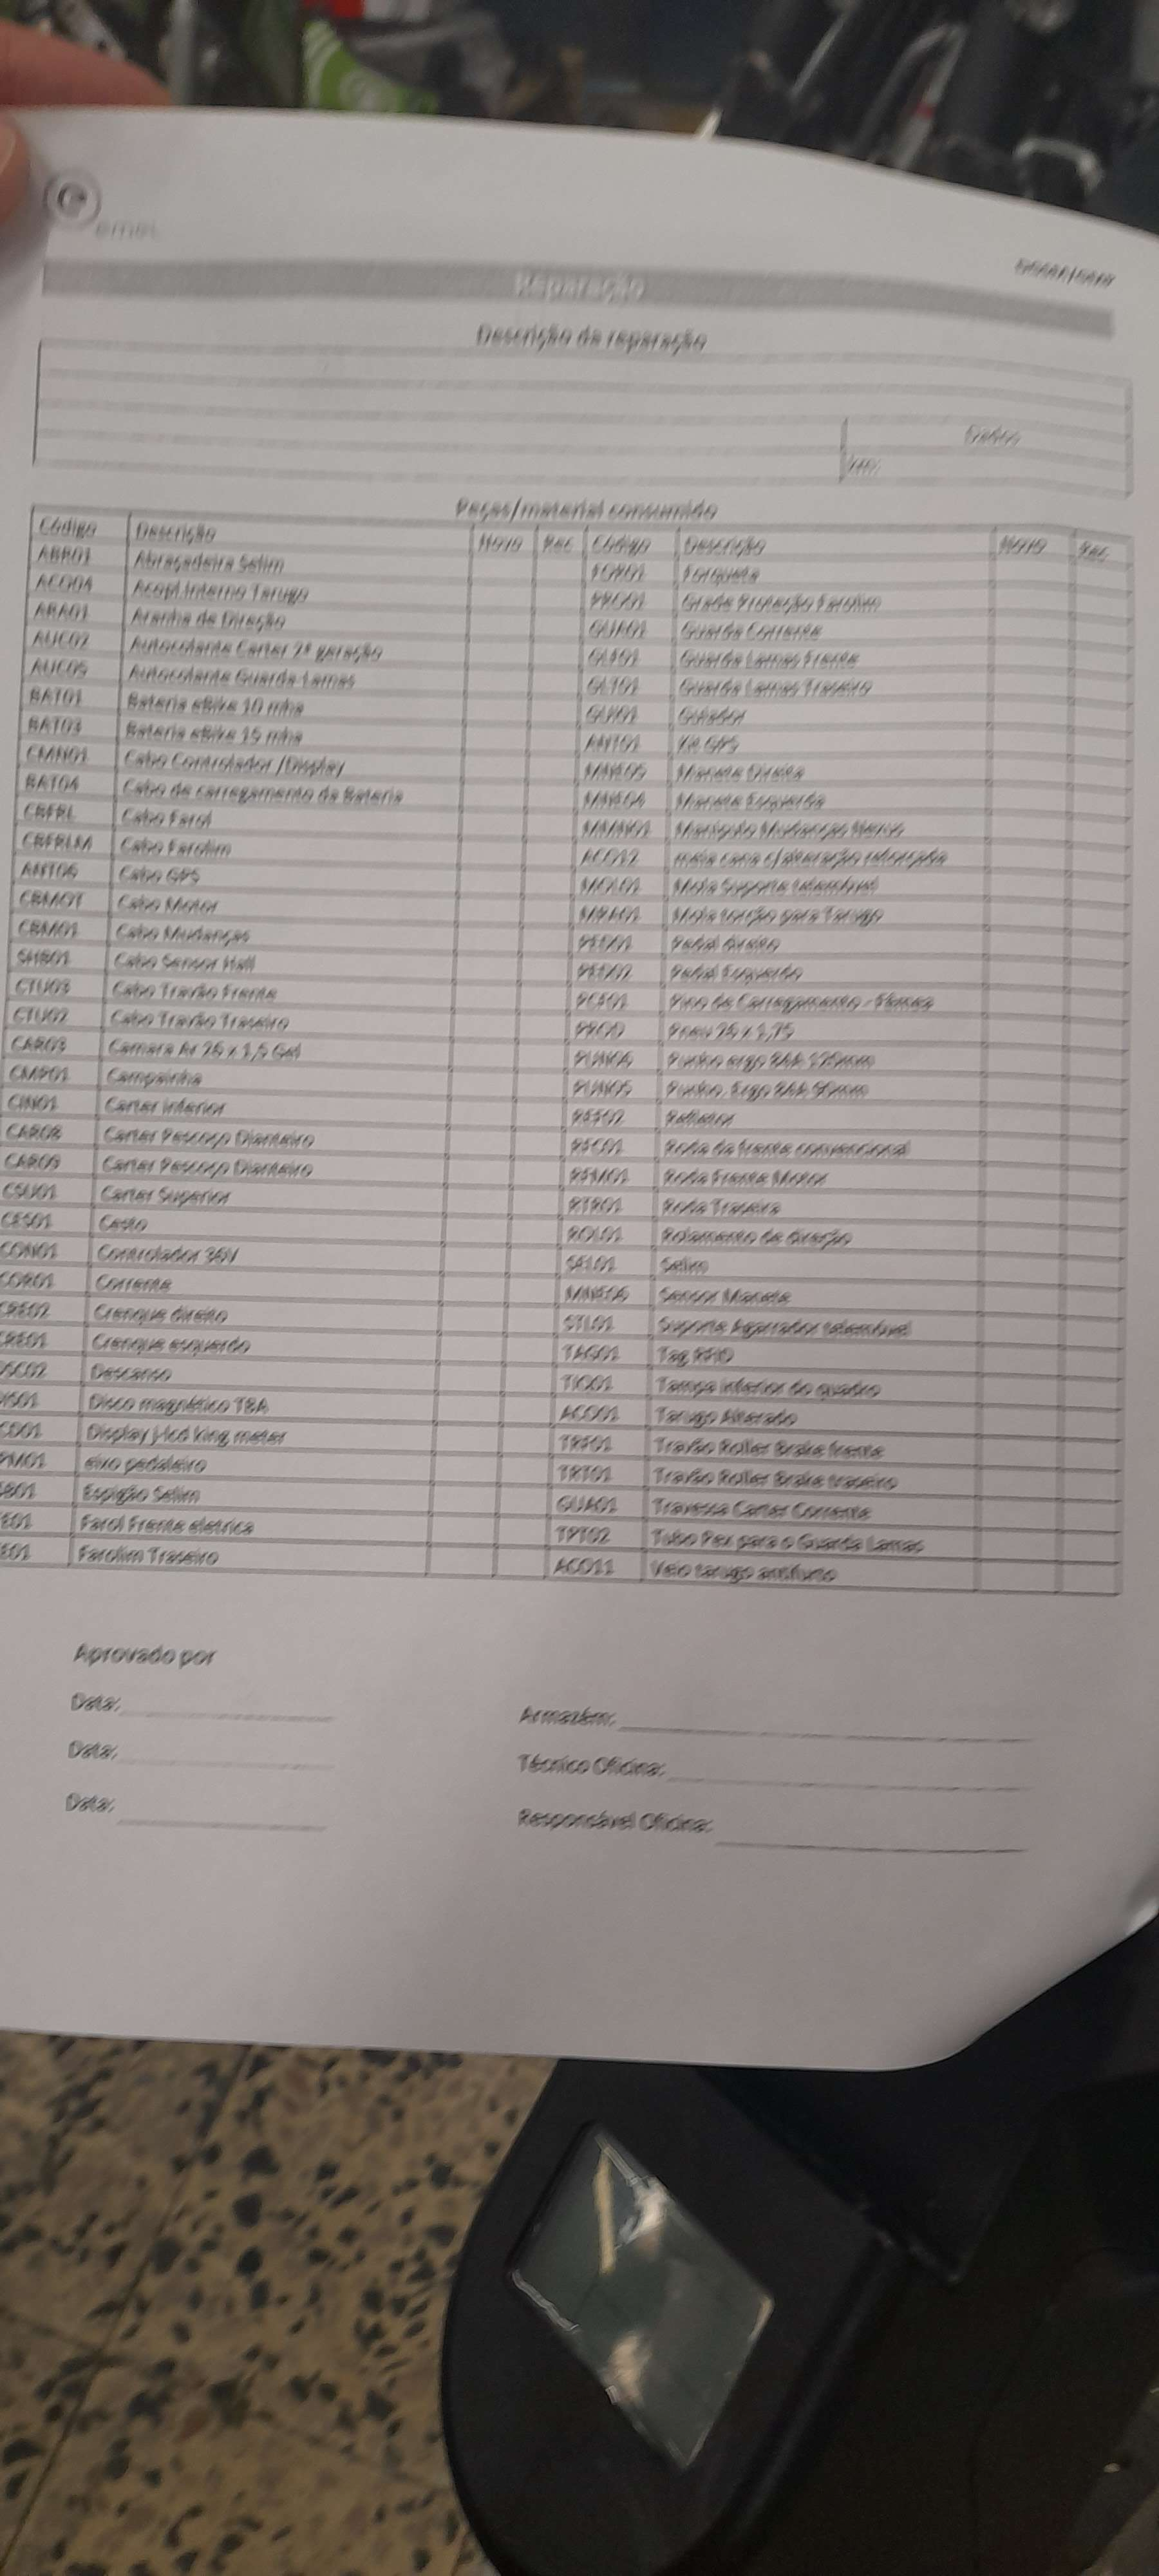
\includegraphics[width=0.50\textwidth]{figs/chapter2/emel_back}
  \label{fig:emel_back}
\end{figure}


\begin{figure}[h]
  \caption{SERVQUAL statements used by the authors in the study to measure the quality of the service at a CMV SA dealership in South Africa (~\cite{Measuring_After_sales_Service_Quality}).}
  \centering
  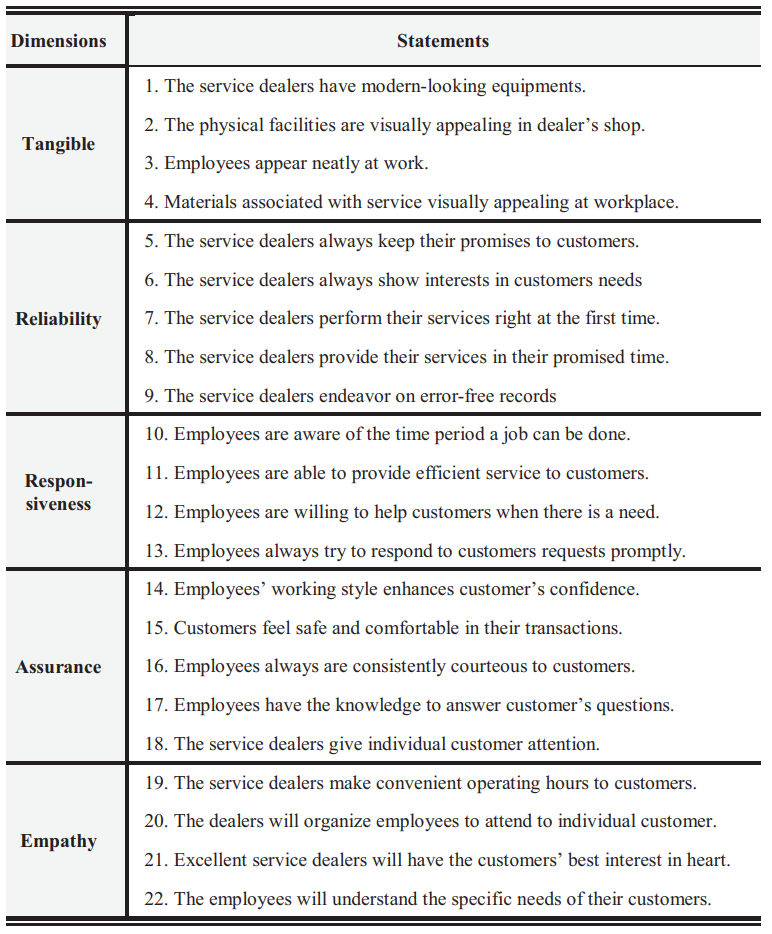
\includegraphics[width=0.75\textwidth]{figs/SERVQUAL_statements}
  \label{fig:SERVQUAL_statements}
\end{figure}


\begin{figure}[h]
  \caption{SERVQUAL results of the study to measure the quality of the service at a CMV SA dealership in South Africa. In the table the header "Exp" means the expectation, "Per" means the perception, "Zc" means the Service quality score from the customers and the "Zc-ms" means Service quality score measure by the difference of the expectations of the customer and the expectation of the dealers. (~\cite{Measuring_After_sales_Service_Quality})}
  \centering
  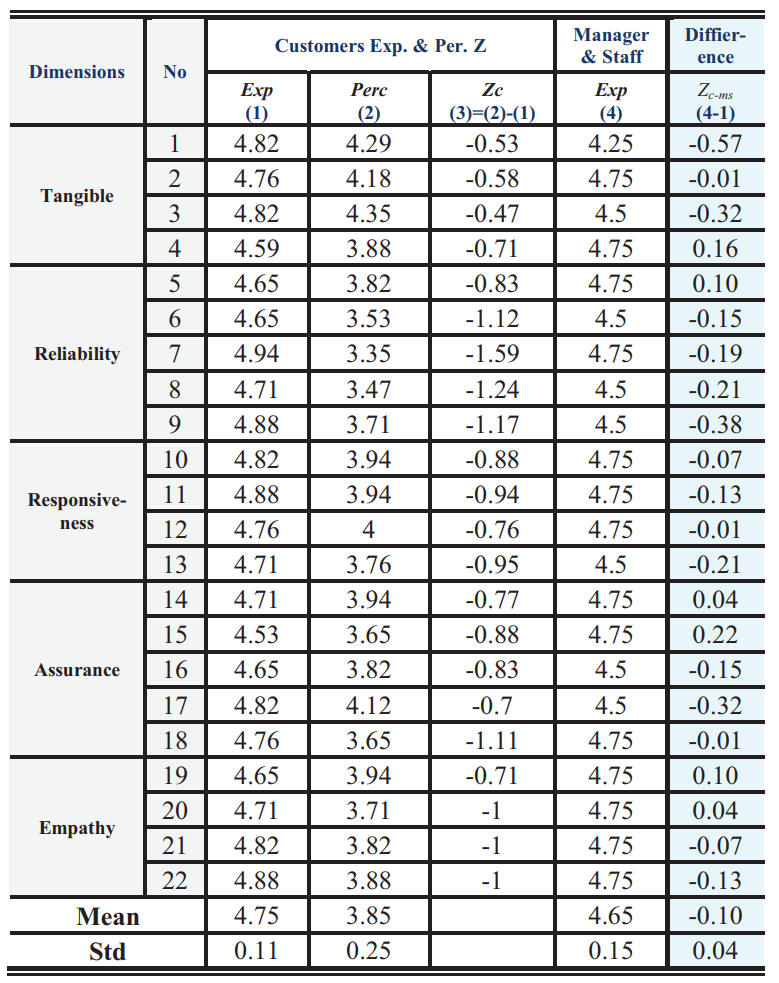
\includegraphics[width=0.75\textwidth]{figs/SERVQUAL_results}
  \label{fig:SERVQUAL_results}
\end{figure}


\begin{figure}[h]
  \caption{Active maintenance details task tab.}
  \centering
  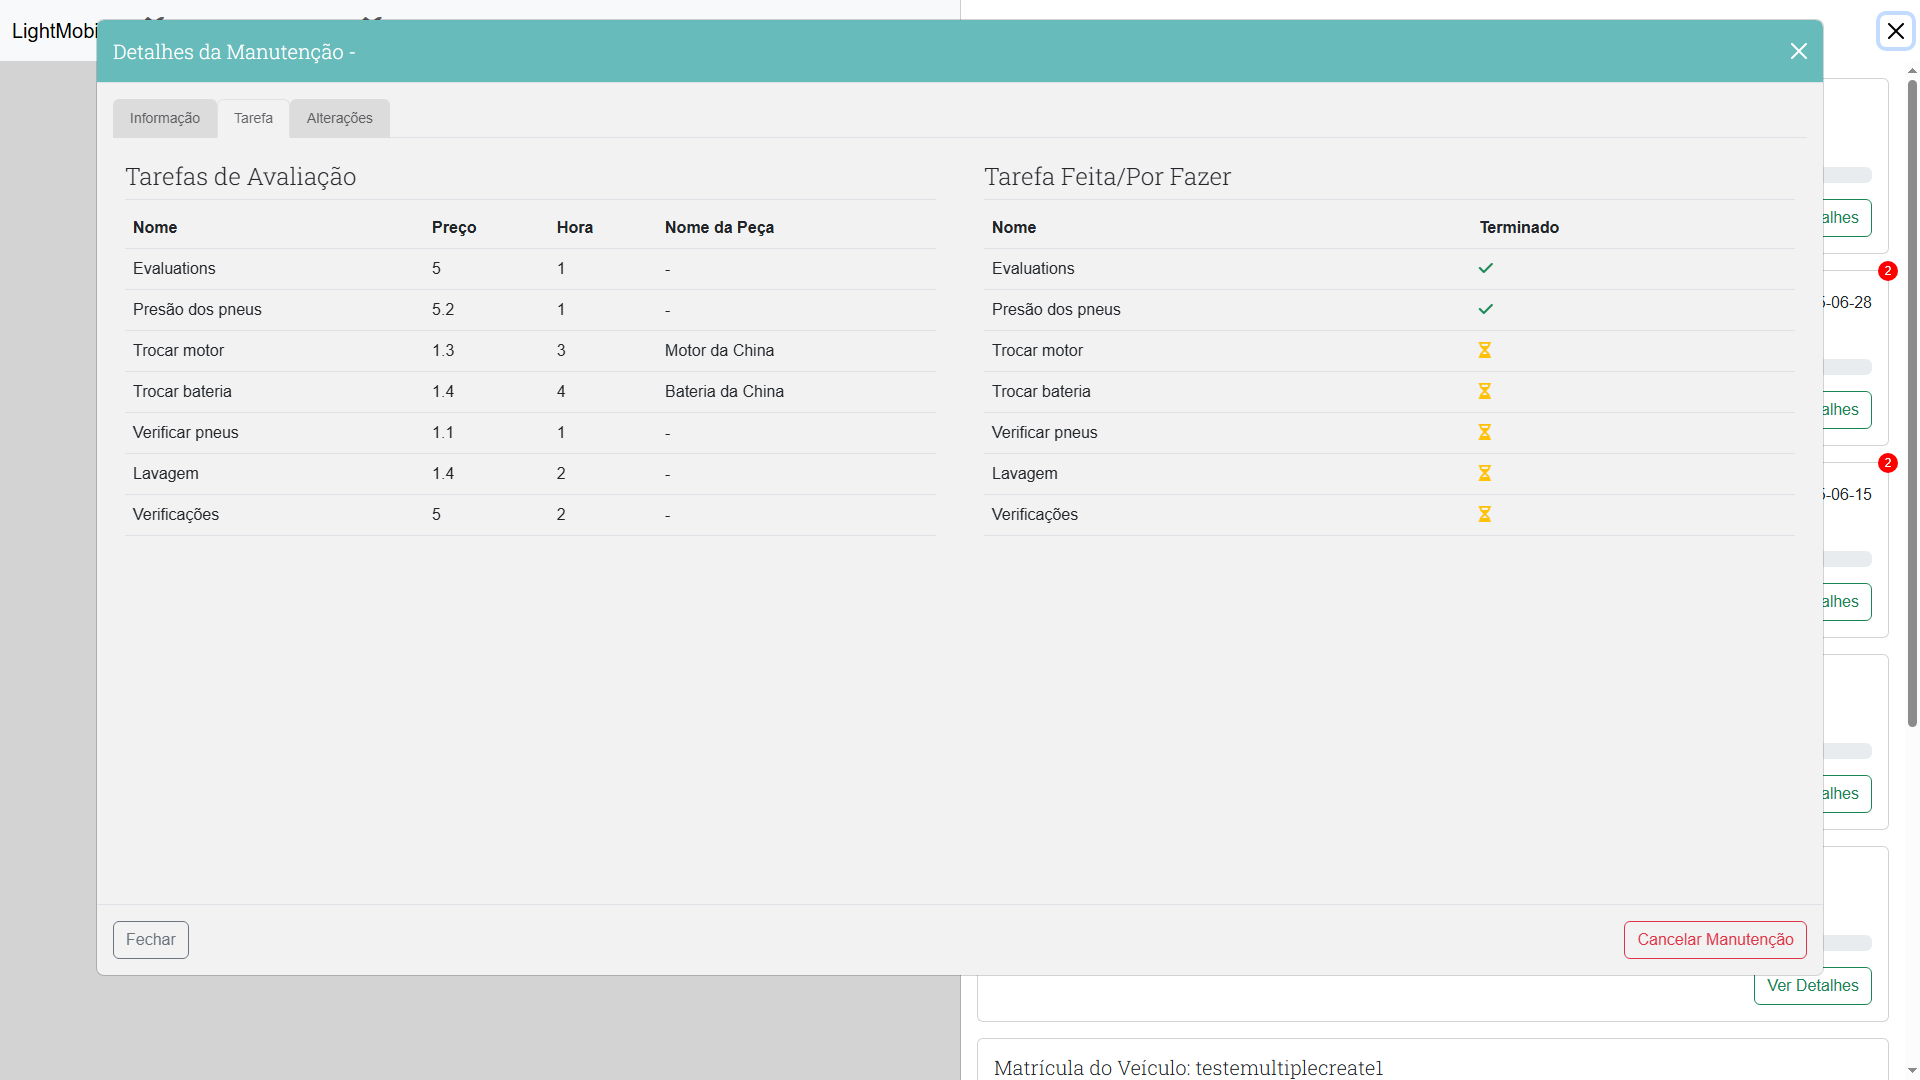
\includegraphics[width=\textwidth]{figs/Implementation/rececionist/maintenance_details_task}
  \label{fig:impReceMaintTask}
\end{figure}


\begin{figure}[h]
  \caption{Active maintenance details change tab.}
  \centering
  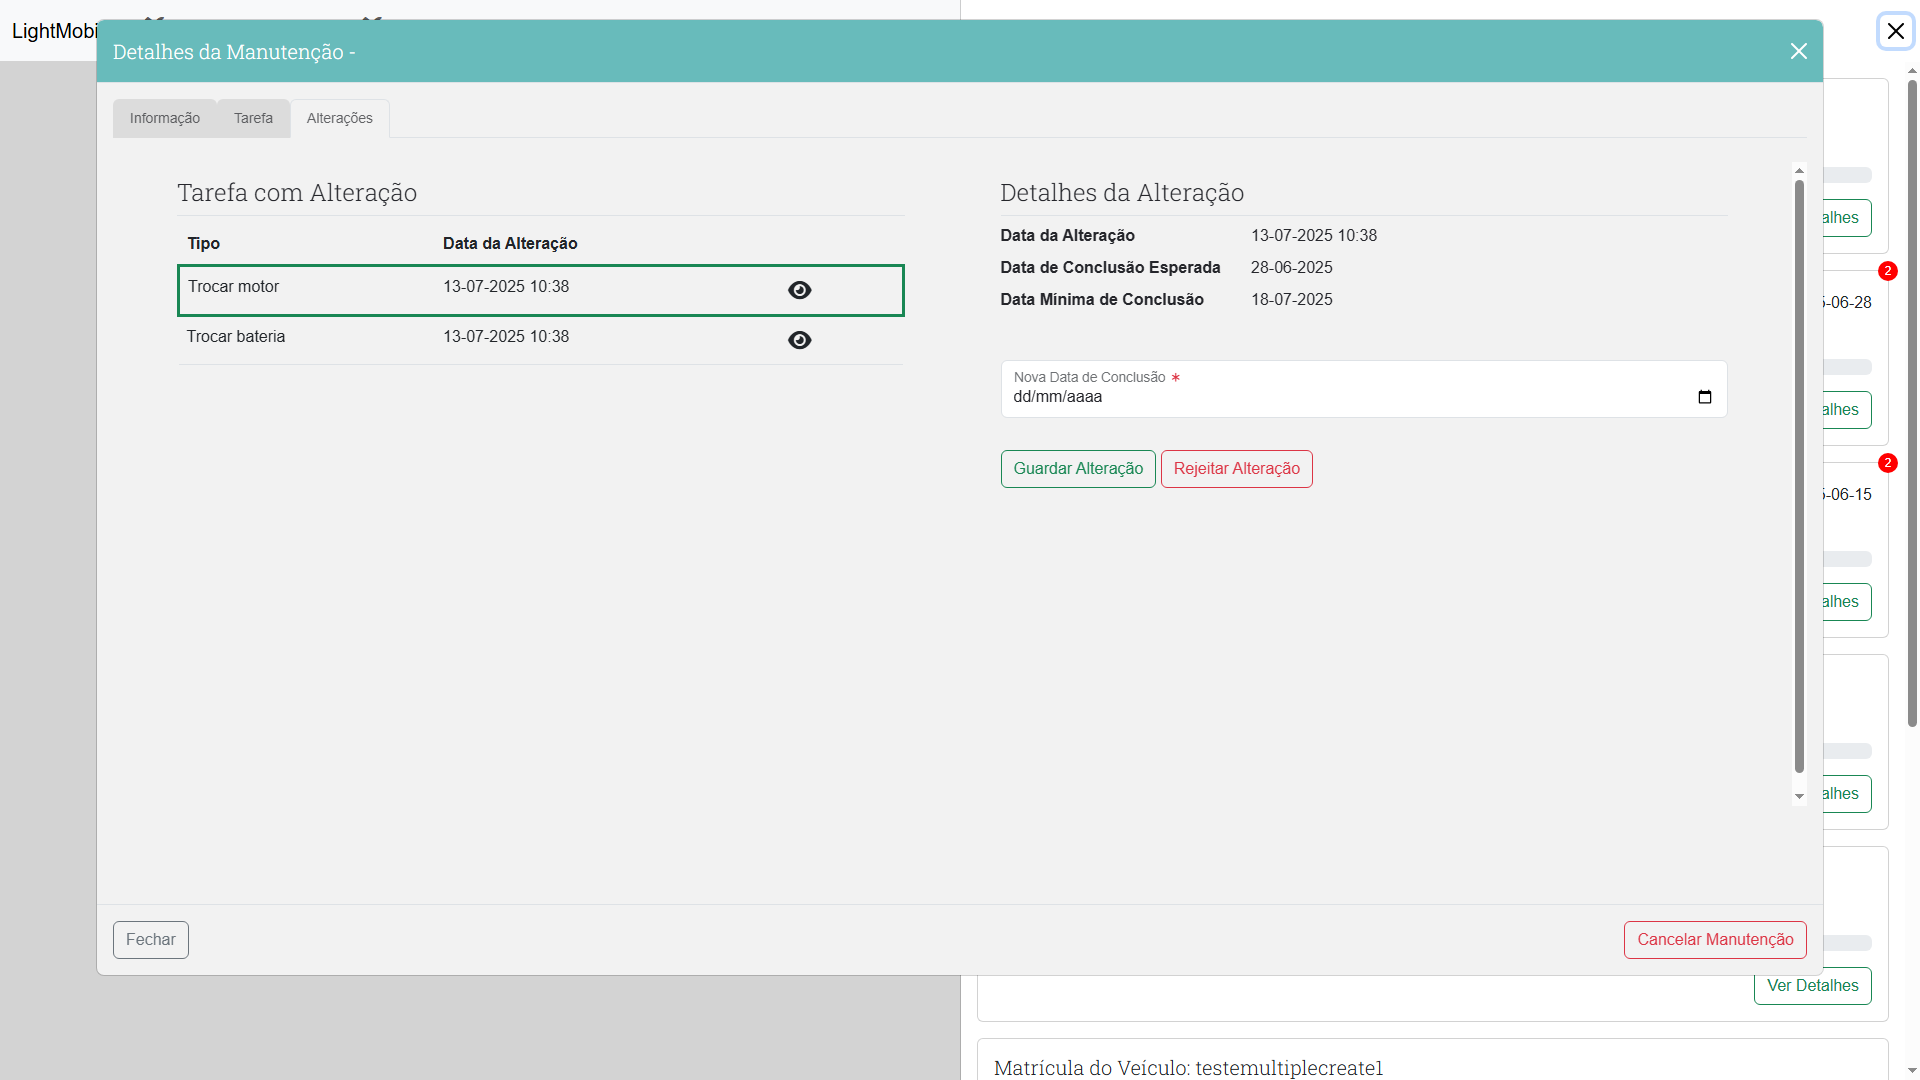
\includegraphics[width=\textwidth]{figs/Implementation/rececionist/maintenance_details_change}
  \label{fig:impReceMaintChange}
\end{figure}



\begin{figure}[h]
  \caption{Mechanic home page with evaluation task.}
  \centering
  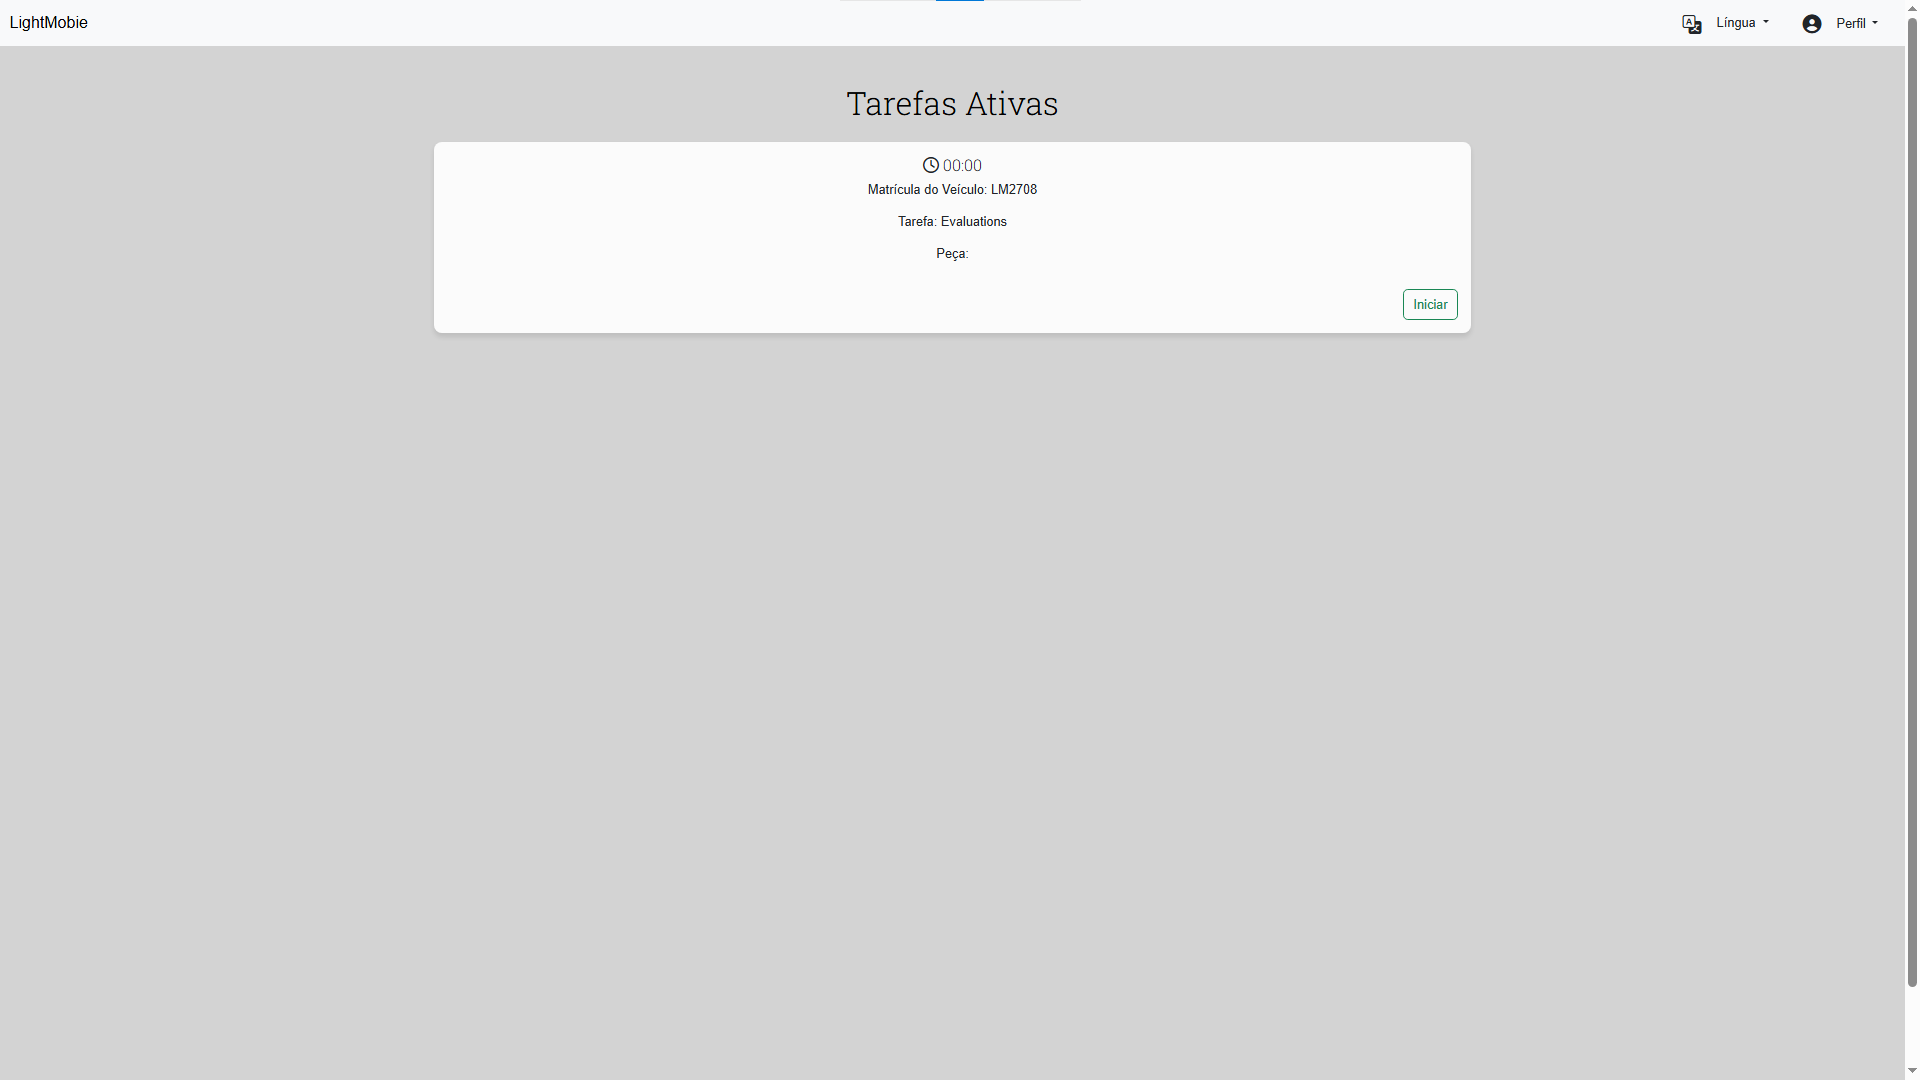
\includegraphics[width=\textwidth]{figs/Implementation/mechanic/HomeEvalNotLate}
  \label{fig:HomeEvalNotLate}
\end{figure}



\begin{figure}[h]
  \caption{Mechanic select part modal.}
  \centering
  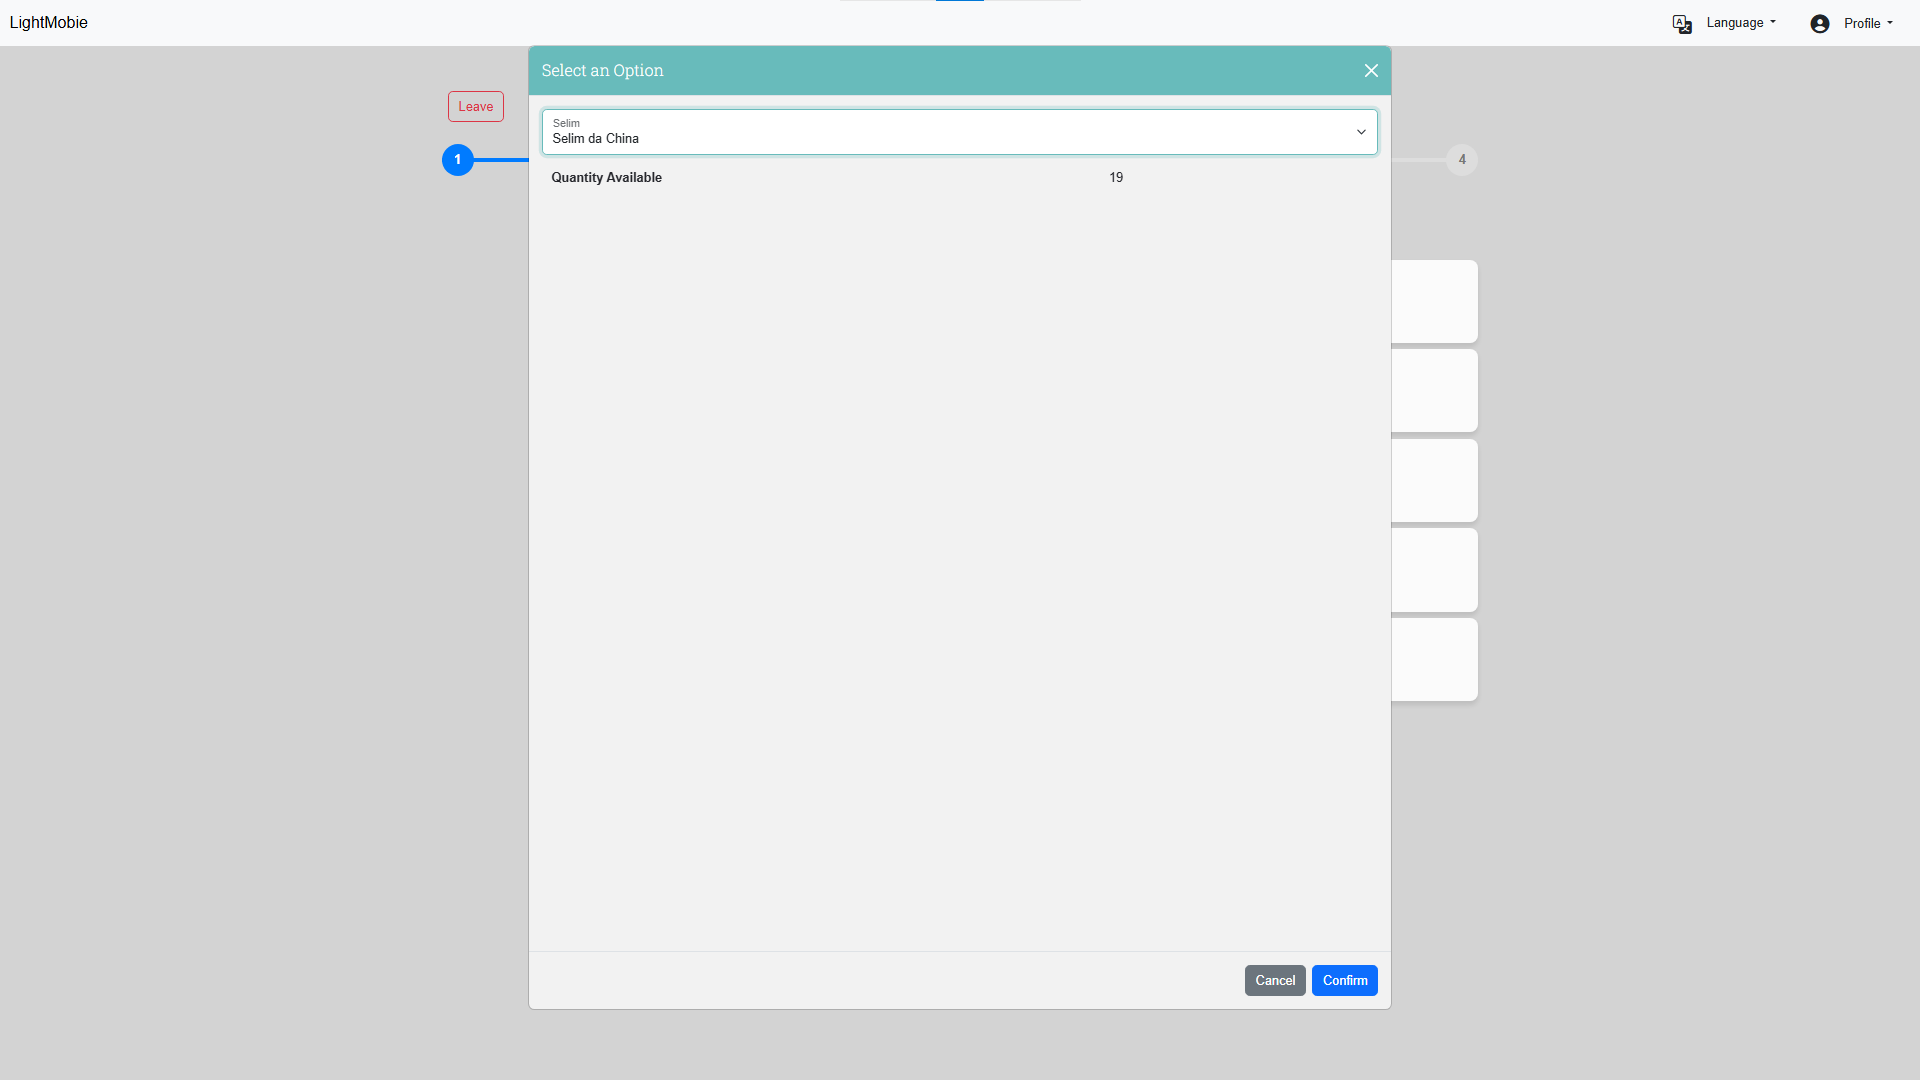
\includegraphics[width=\textwidth]{figs/Implementation/mechanic/MechanicEvaluationSelectTaskWitPart}
  \label{fig:MechanicEvaluationSelectTaskWitPart}
\end{figure}

\begin{figure}[h]
  \caption{Mechanic Evaluation task with part selected.}
  \centering
  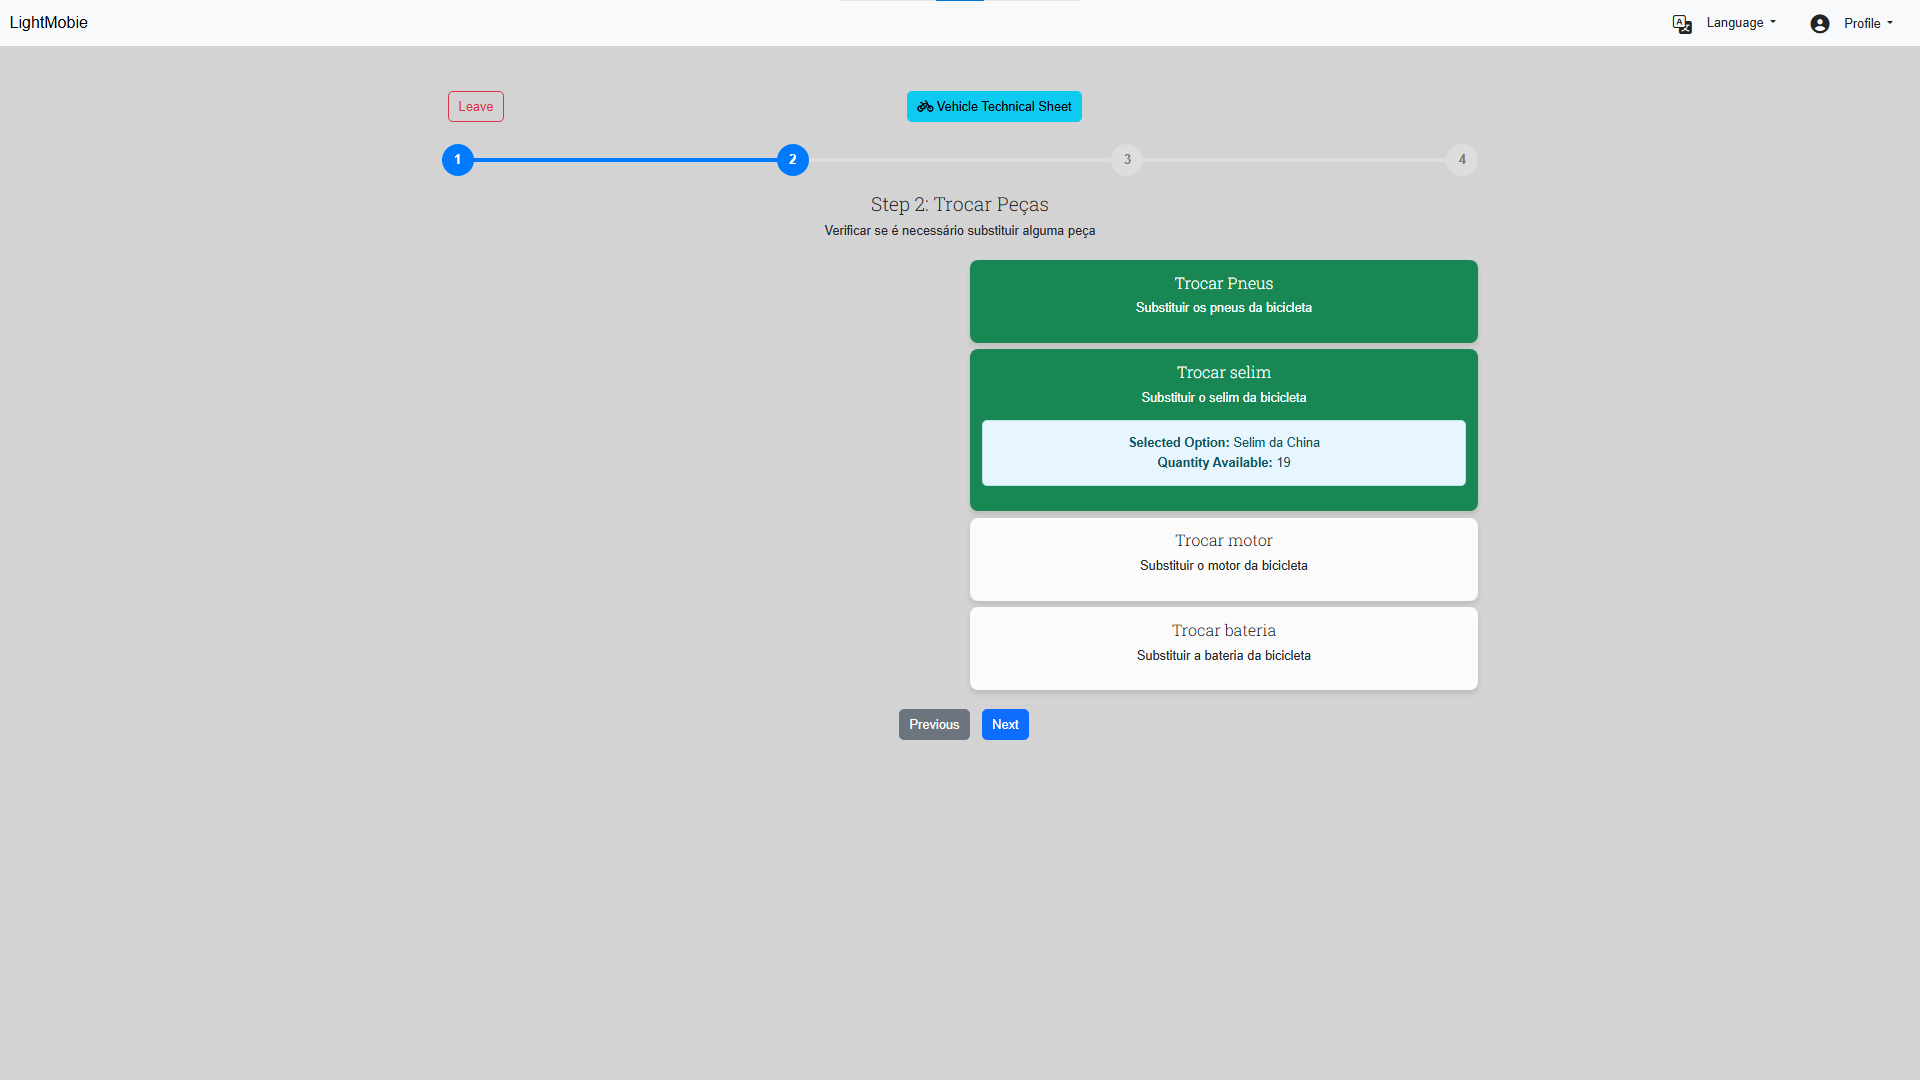
\includegraphics[width=\textwidth]{figs/Implementation/mechanic/TaskSelected}
  \label{fig:TaskSelected}
\end{figure}




\begin{figure}[h]
  \caption{Inventory editor.}
  \centering
  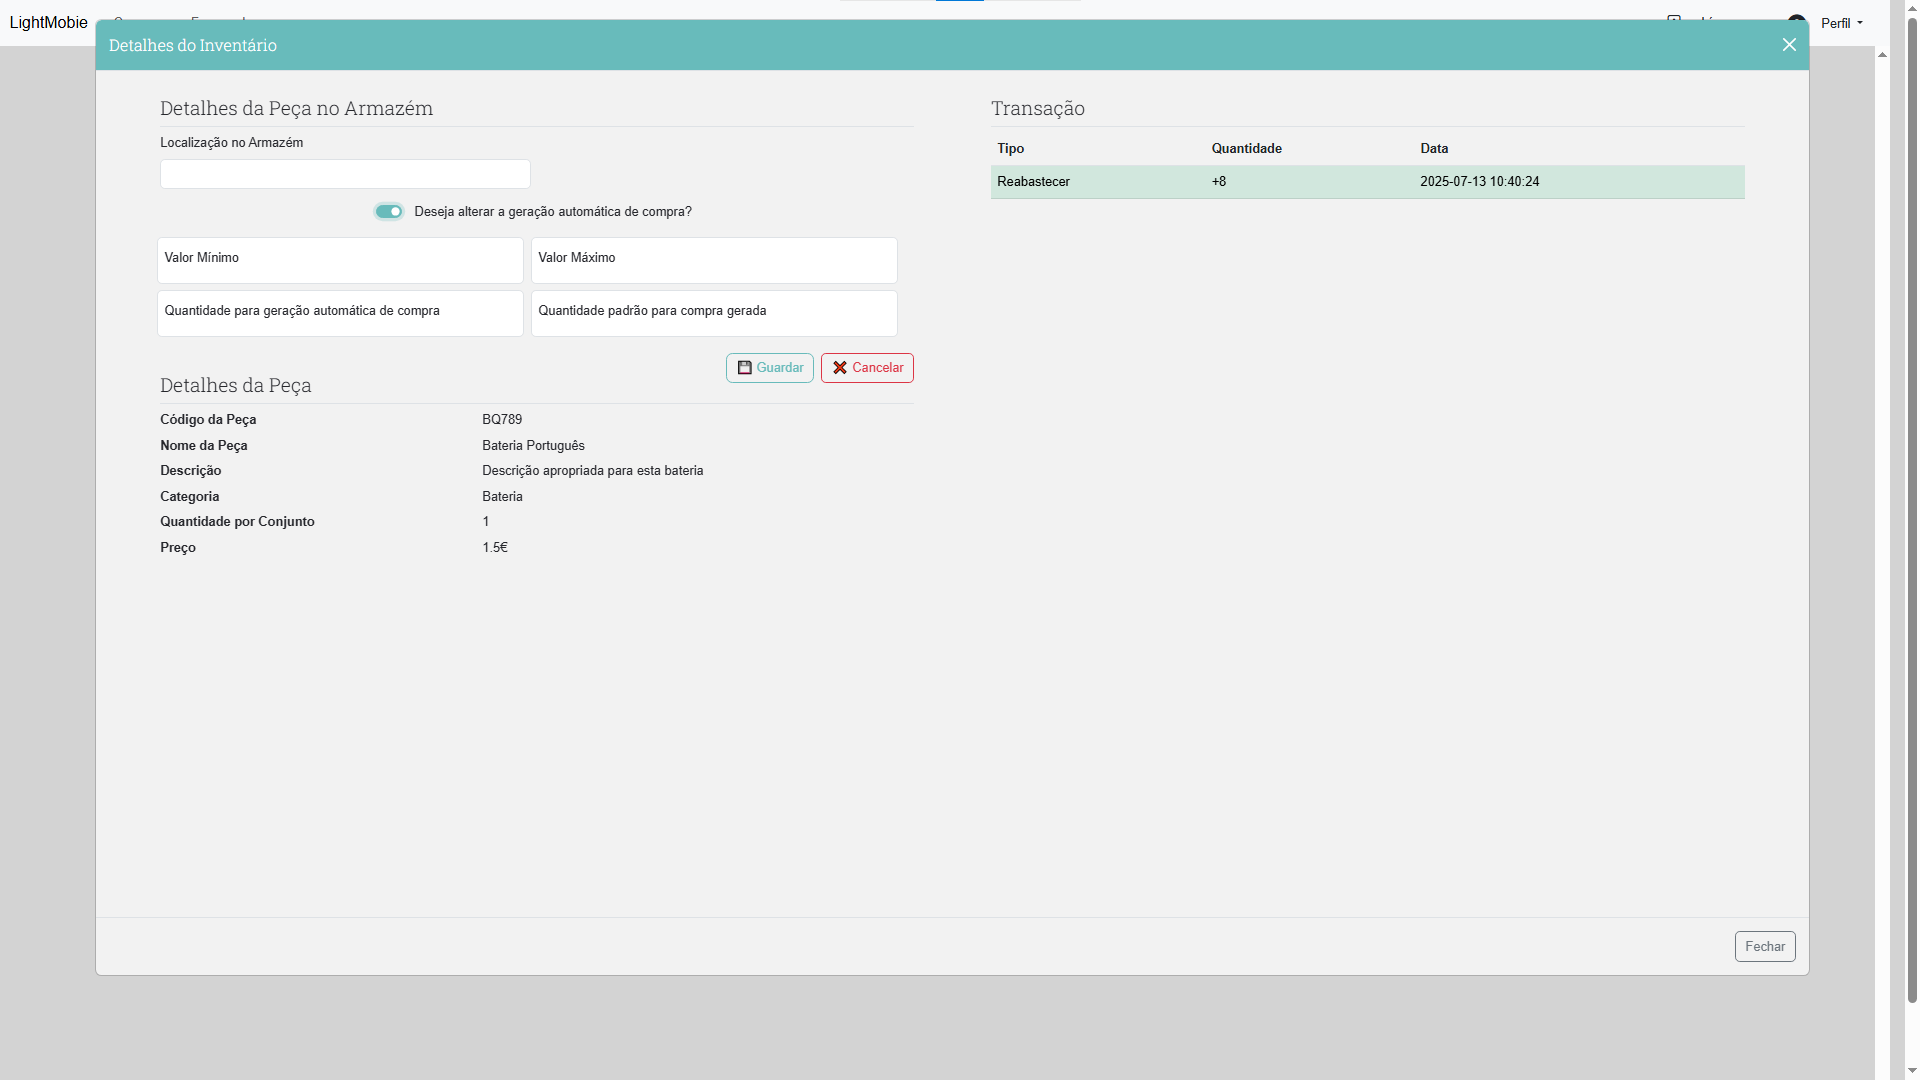
\includegraphics[width=\textwidth]{figs/Implementation/warehouse/inventoryEdit}
  \label{fig:inventoryEdit}
\end{figure}



\begin{figure}[h]
  \caption{Create new purchase modal with a part selected.}
  \centering
  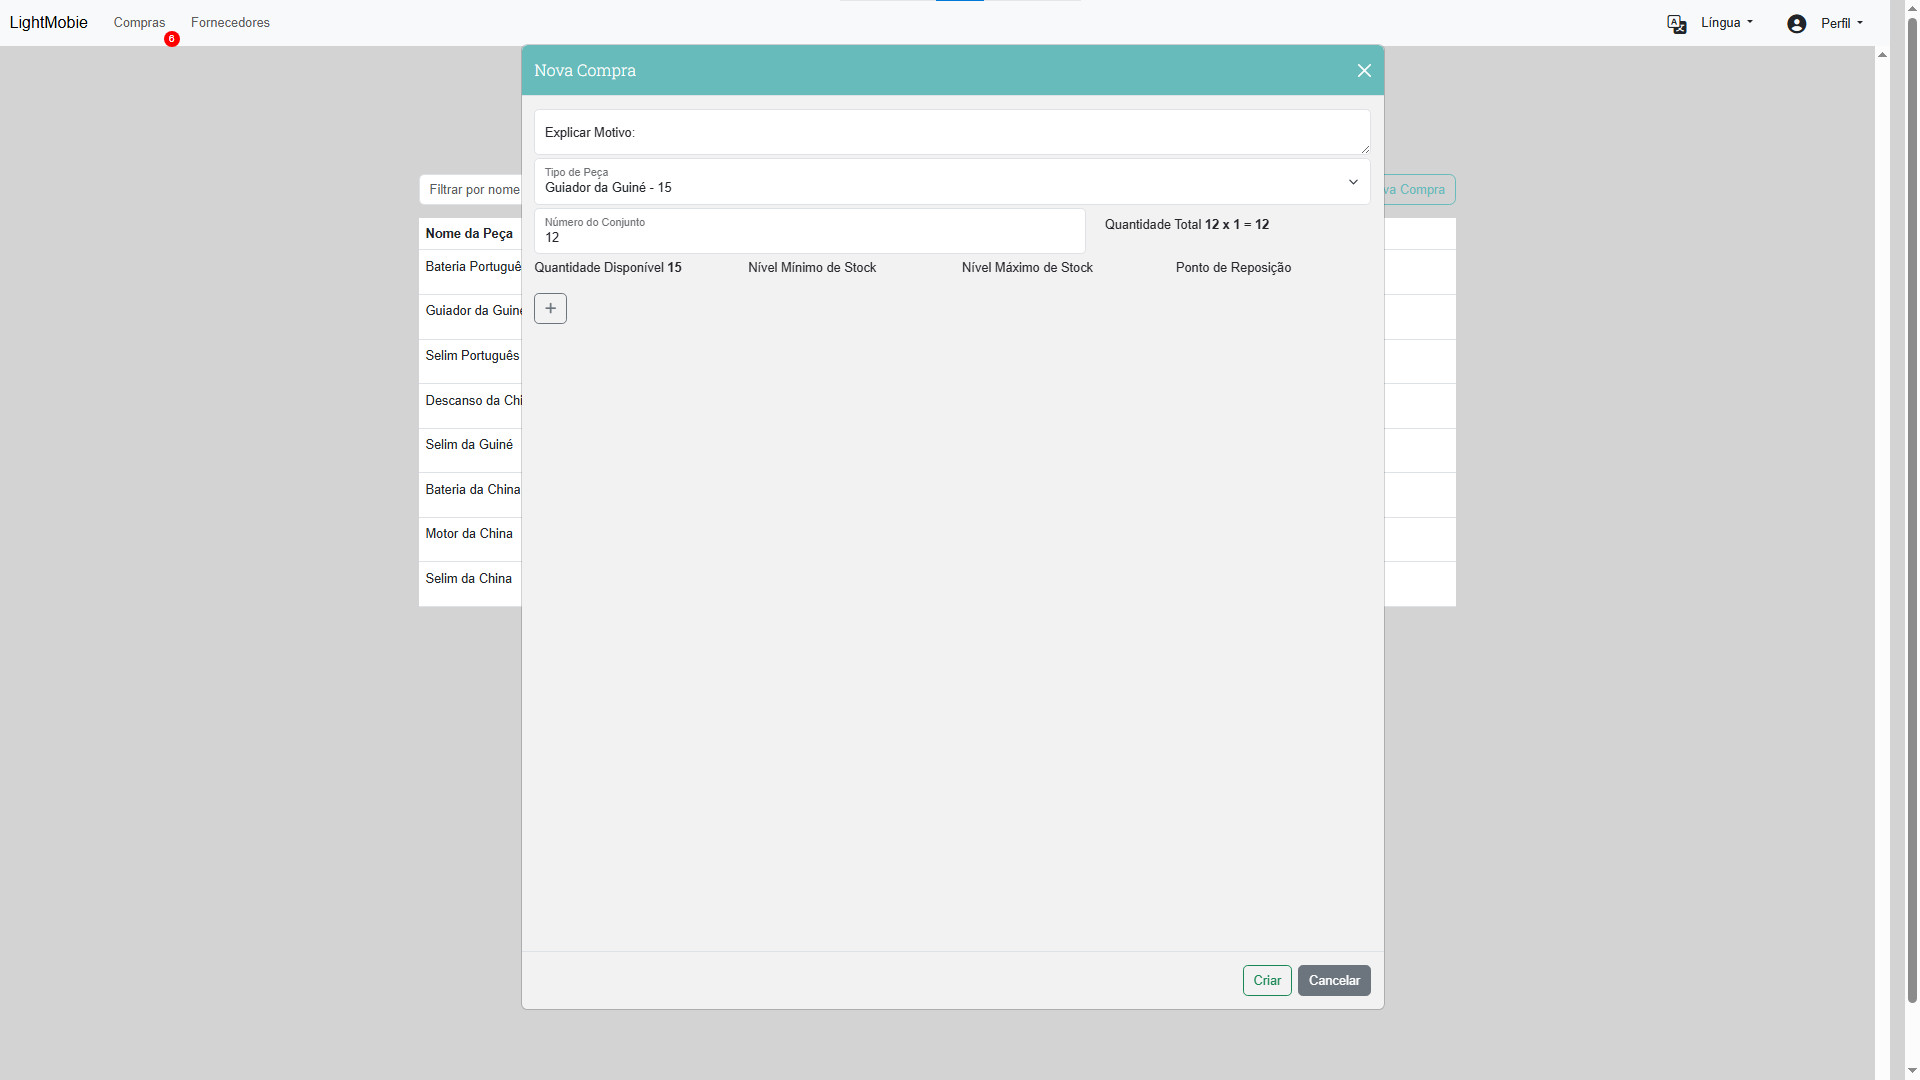
\includegraphics[width=\textwidth]{figs/Implementation/warehouse/createPurchaseWithParts}
  \label{fig:createPurchaseWithParts}
\end{figure}

\begin{figure}[h]
  \caption{Create new purchase modal with a part added.}
  \centering
  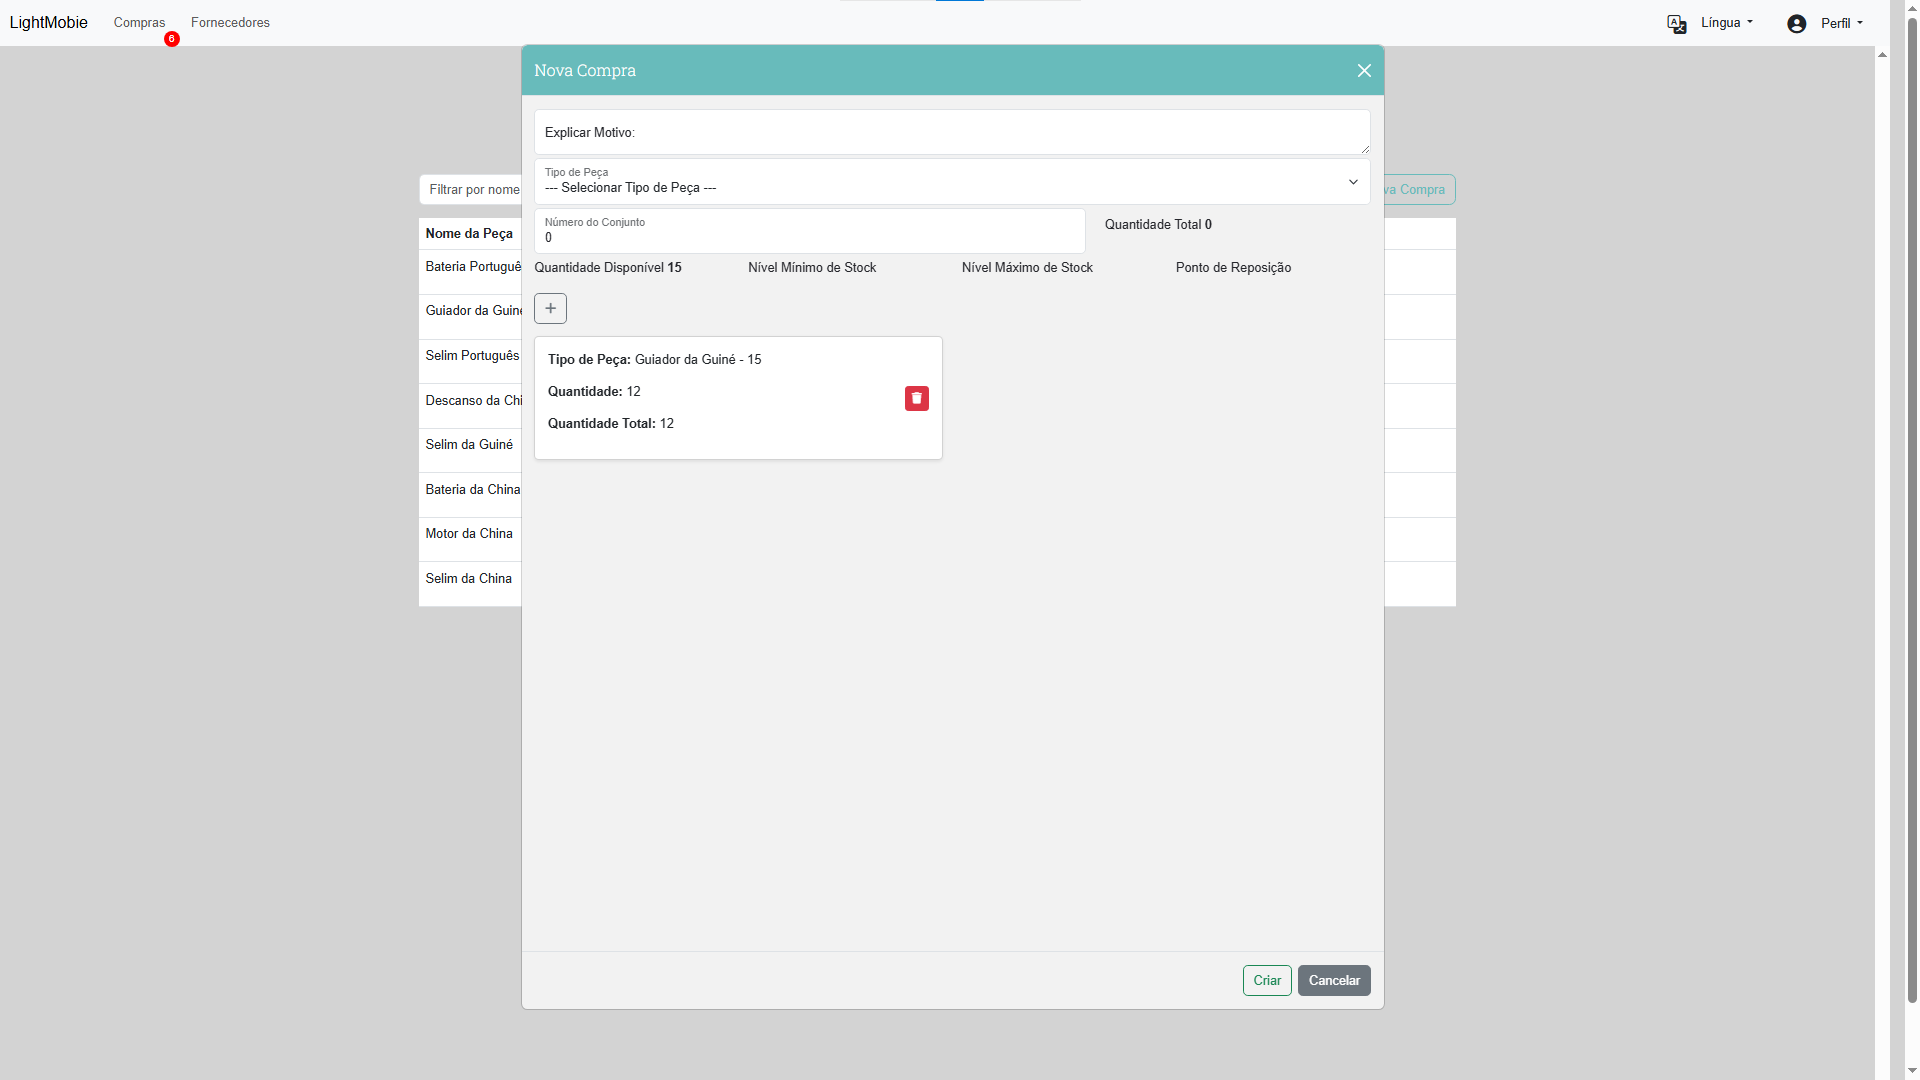
\includegraphics[width=\textwidth]{figs/Implementation/warehouse/createPurchaseAddedPart}
  \label{fig:createPurchaseAddedPart}
\end{figure}



\begin{figure}[h]
  \caption{Waiting delivery purchase details.}
  \centering
  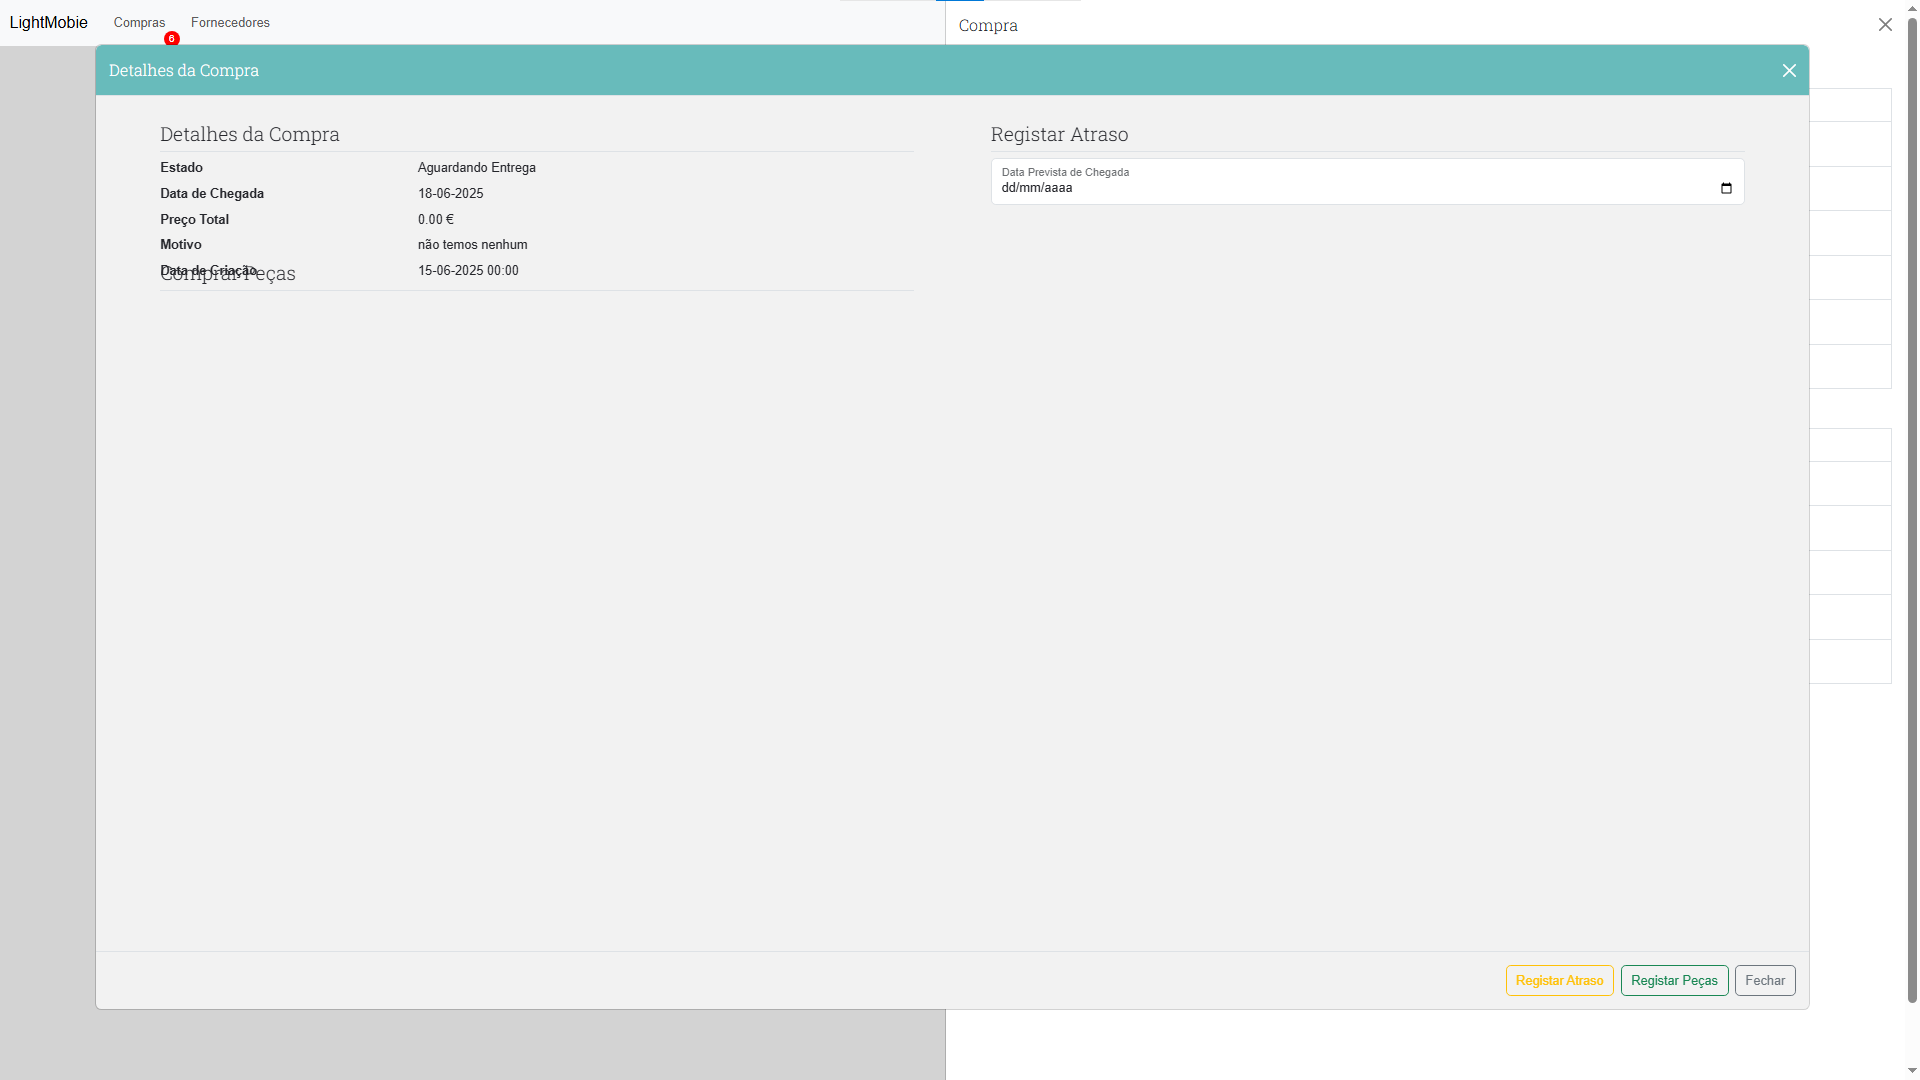
\includegraphics[width=\textwidth]{figs/Implementation/warehouse/PurchaseRegisterParts}
  \label{fig:PurchaseRegisterParts}
\end{figure}


\begin{figure}[h]
  \caption{Delivered purchase details.}
  \centering
  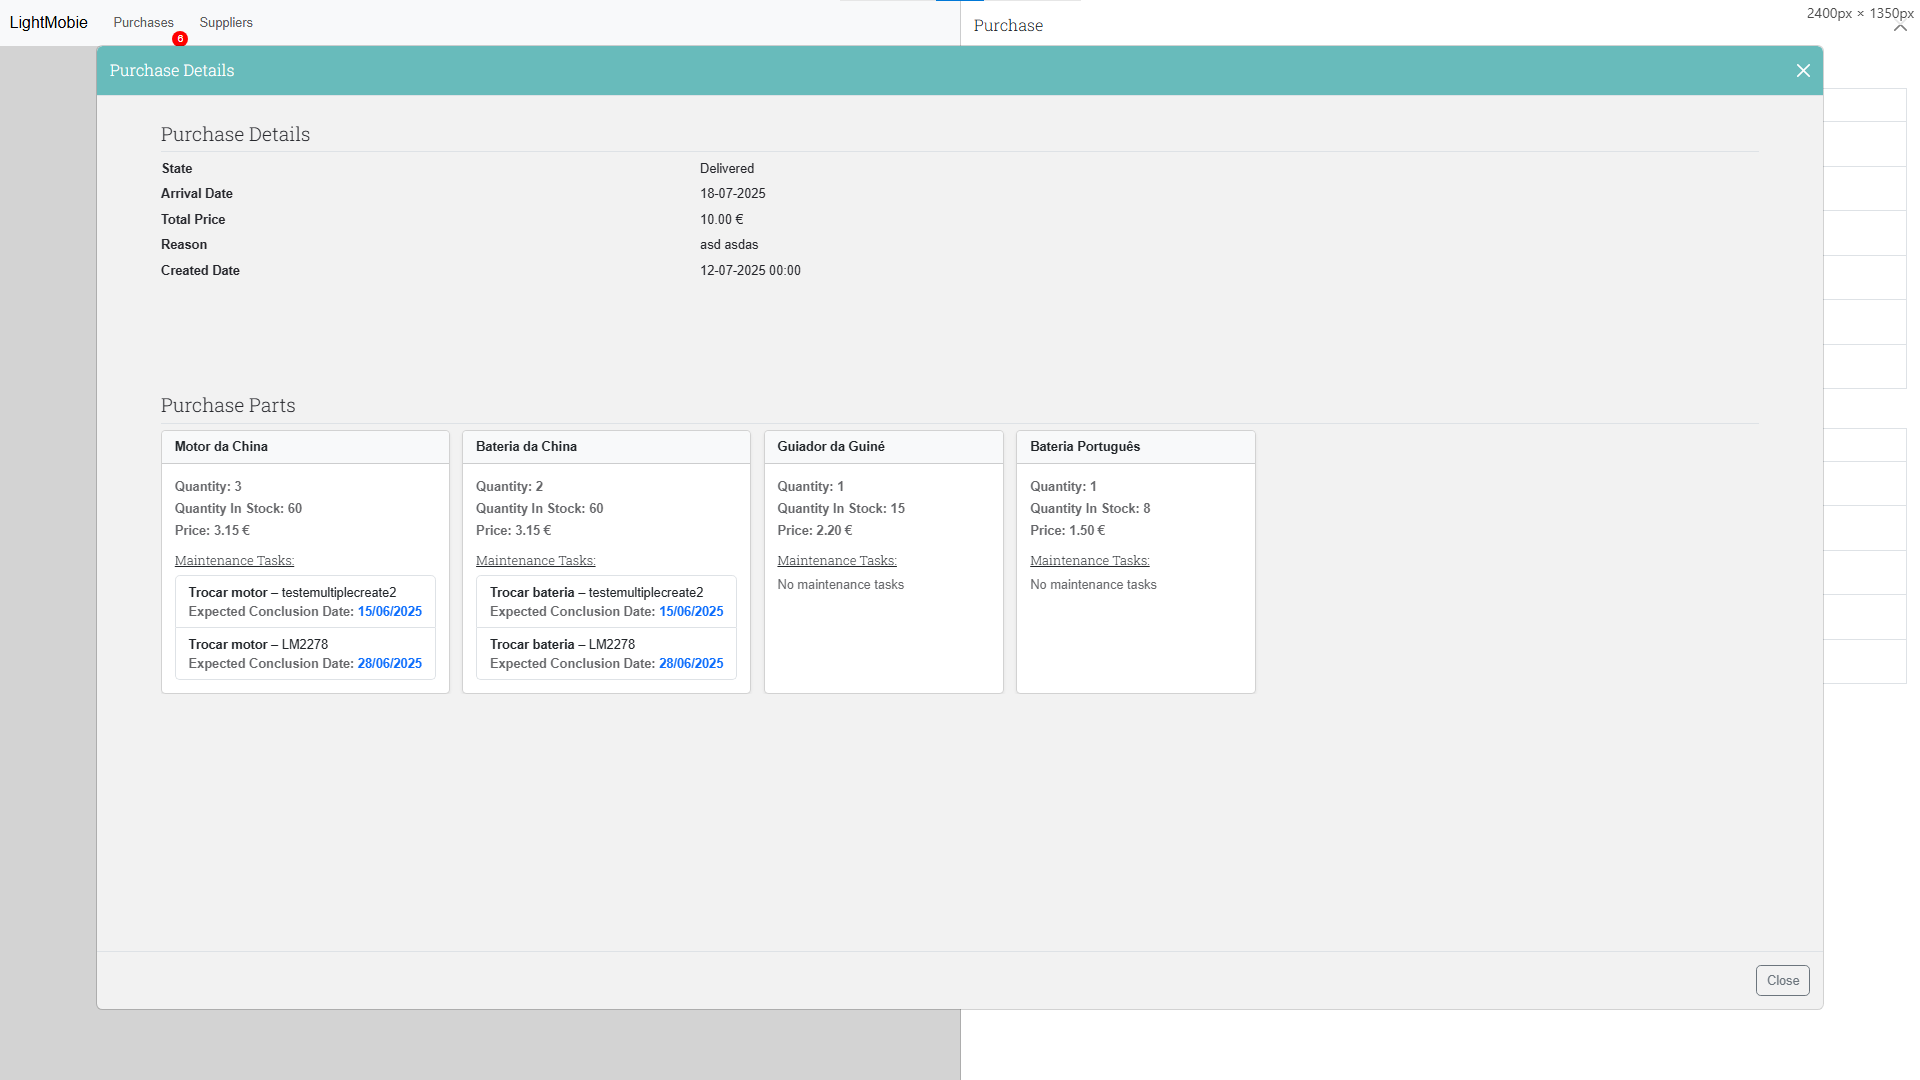
\includegraphics[width=\textwidth]{figs/Implementation/warehouse/PurchaseFinishedDetails}
  \label{fig:PurchaseFinishedDetails}
\end{figure}


\begin{figure}[h]
  \caption{Active maintenance list.}
  \centering
  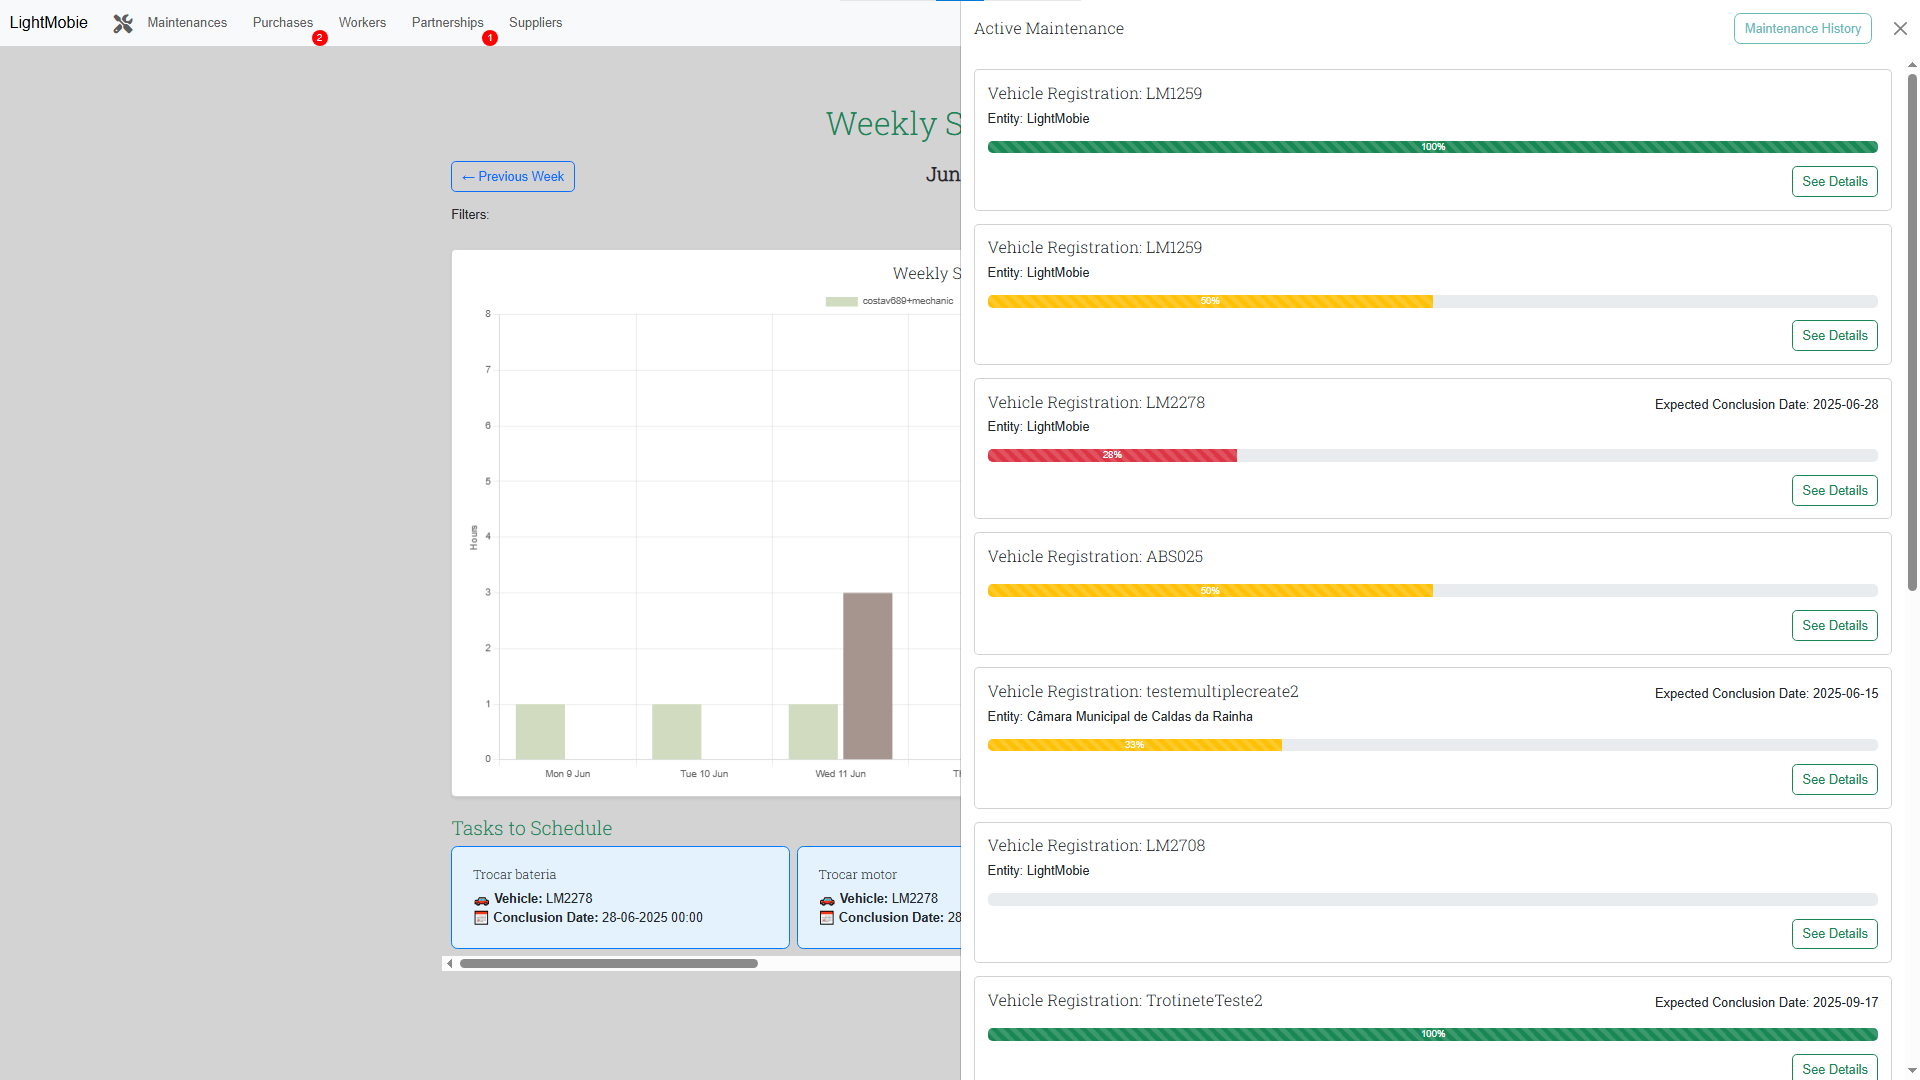
\includegraphics[width=\textwidth]{figs/Implementation/workshopmanager/maintenanceList}
  \label{fig:workshopmanagerMaintenanceList}
\end{figure}


\begin{figure}[h]
  \caption{Maintenance details information tab.}
  \centering
  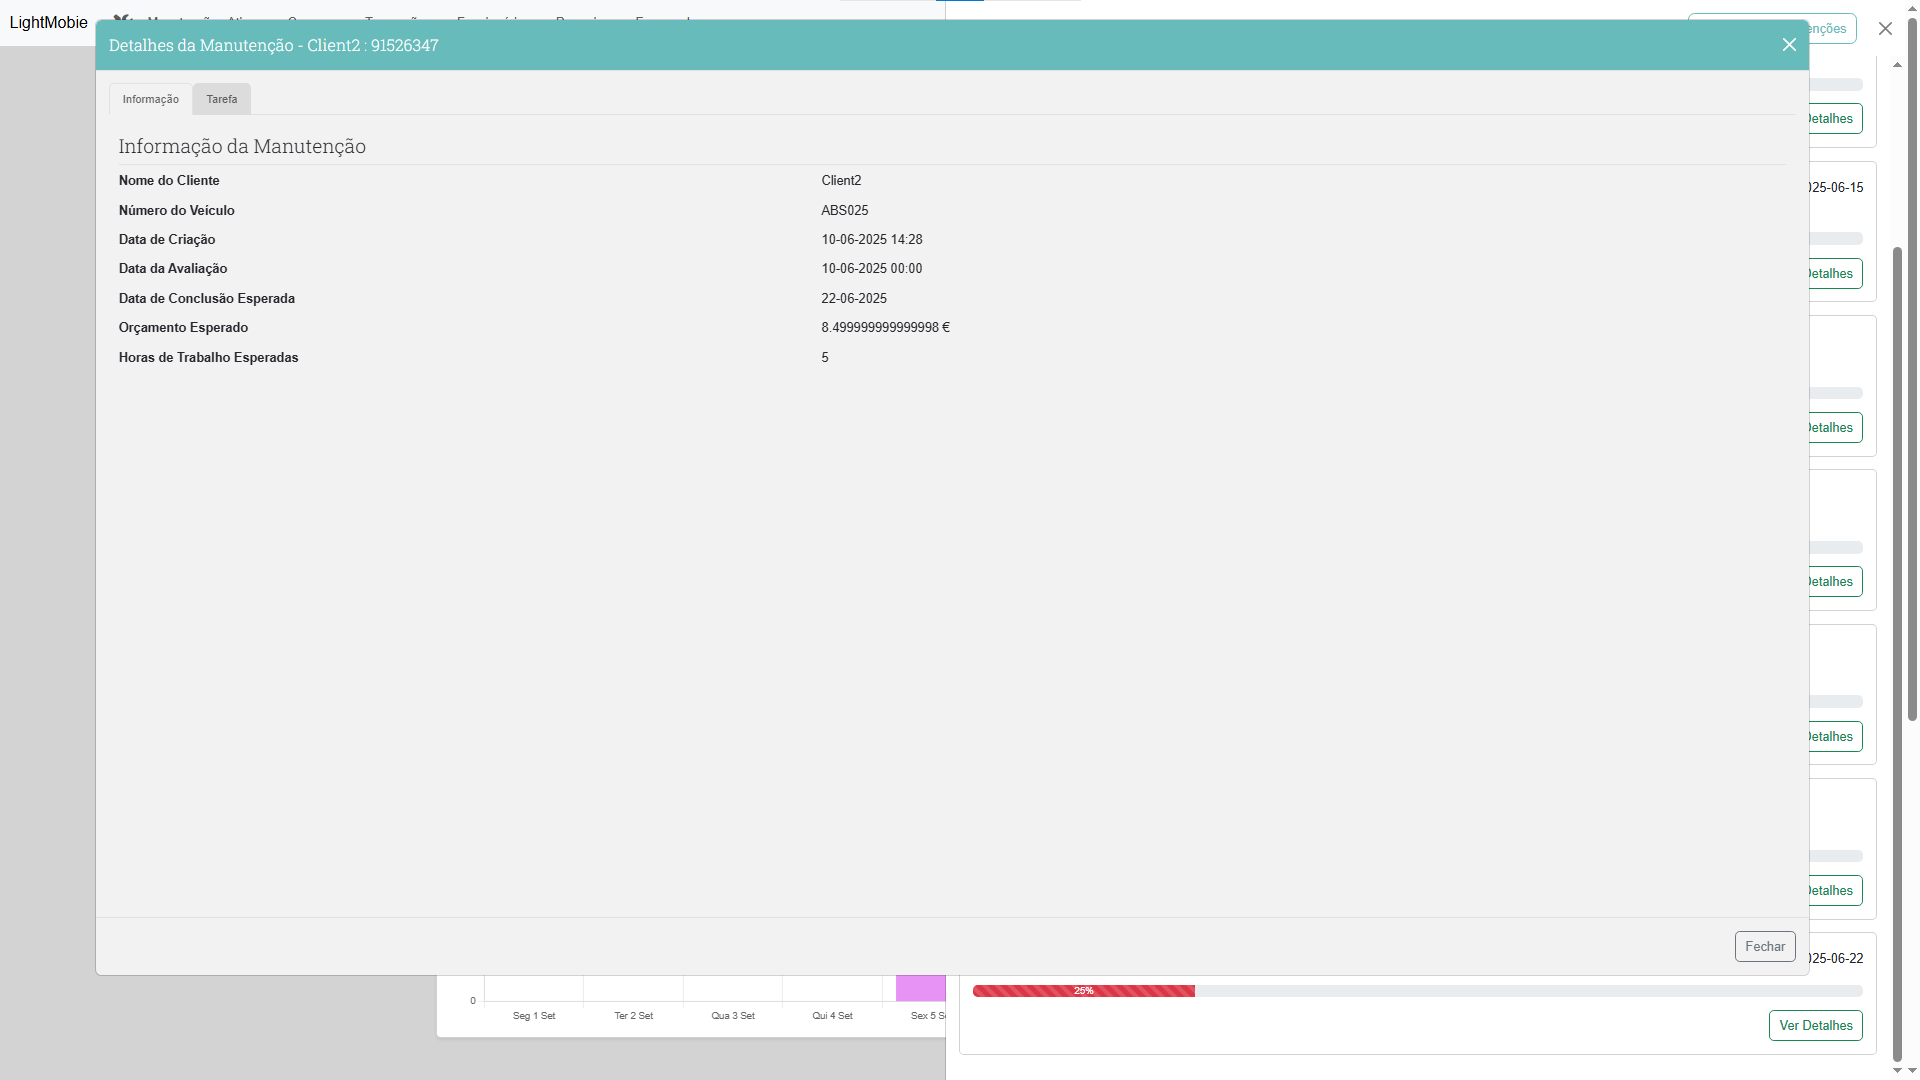
\includegraphics[width=\textwidth]{figs/Implementation/workshopmanager/maintenanceDetails}
  \label{fig:workshopmanagerMaintenanceDetails}
\end{figure}




\begin{figure}[h]
  \caption{Supplier list.}
  \centering
  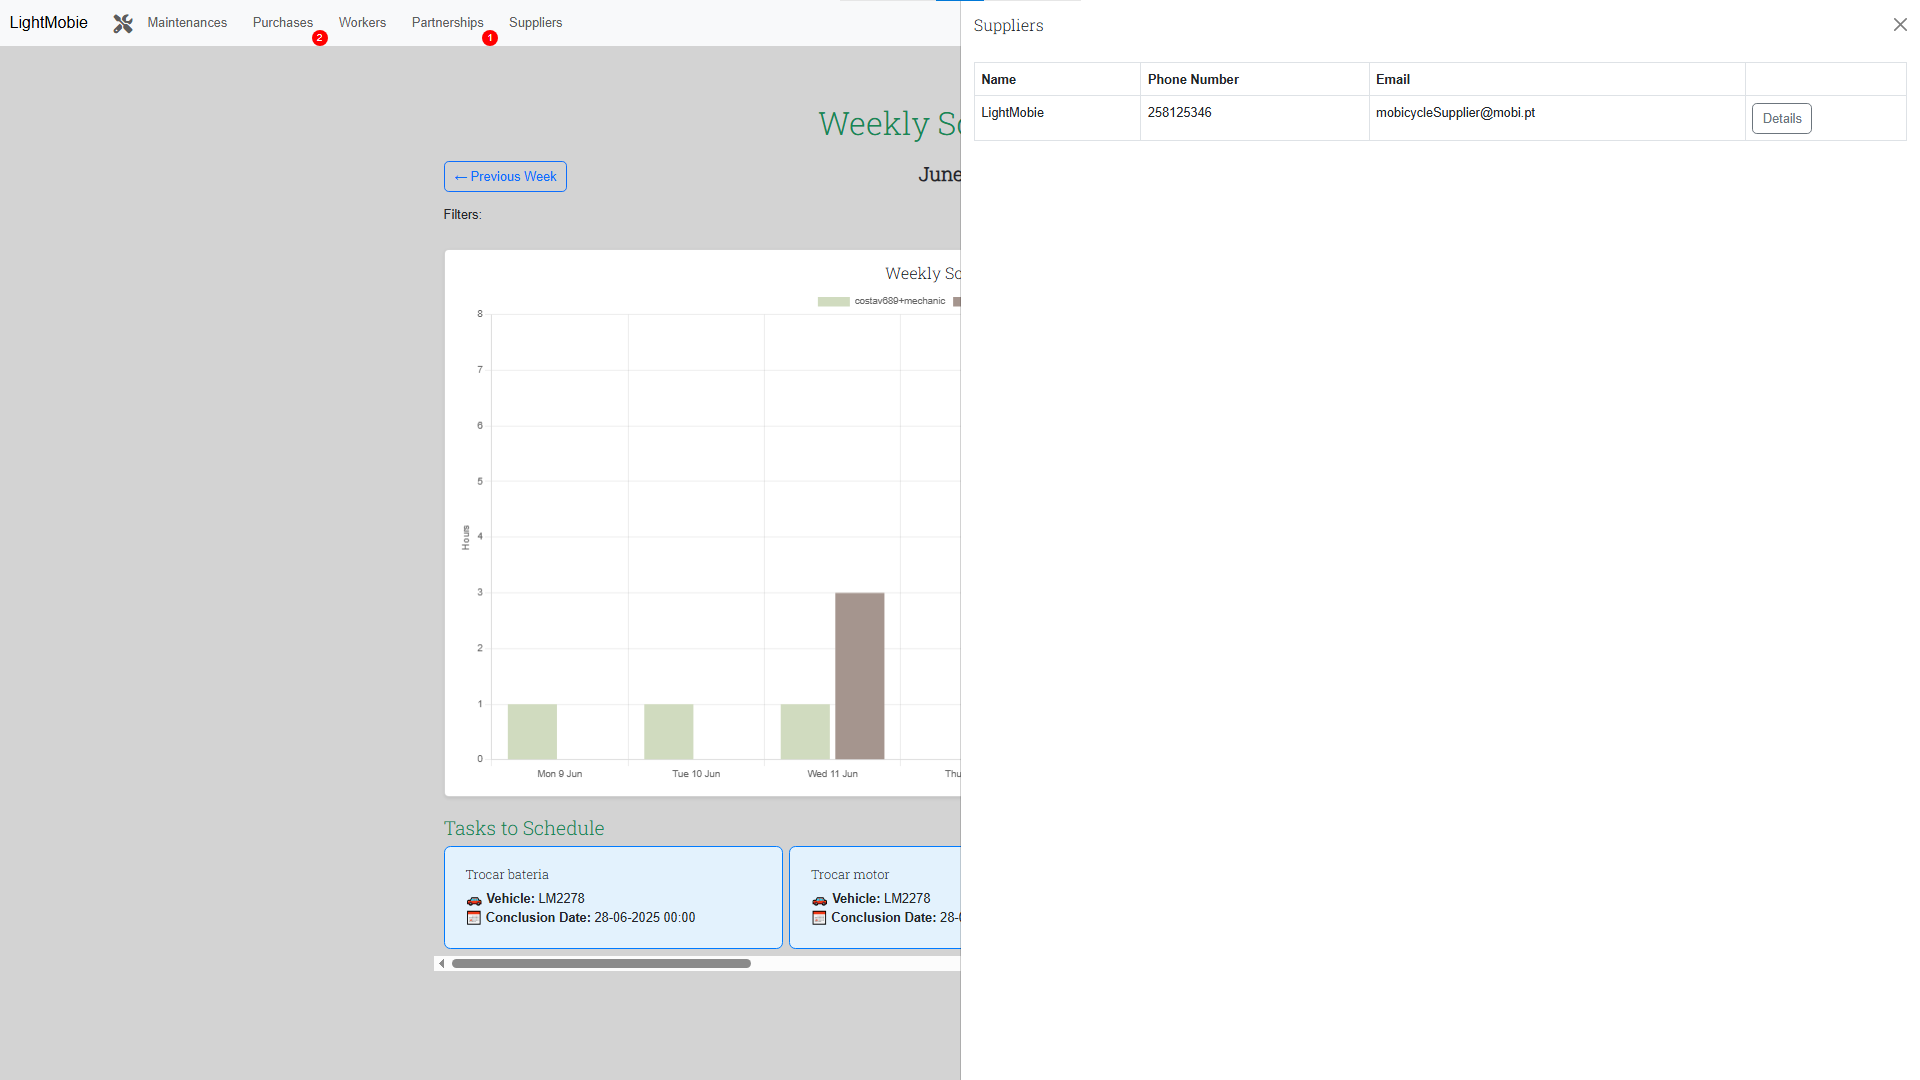
\includegraphics[width=\textwidth]{figs/Implementation/workshopmanager/supplierList}
  \label{fig:workshopmanagerSupplierList}
\end{figure}

\begin{figure}[h]
  \caption{Supplier Details.}
  \centering
  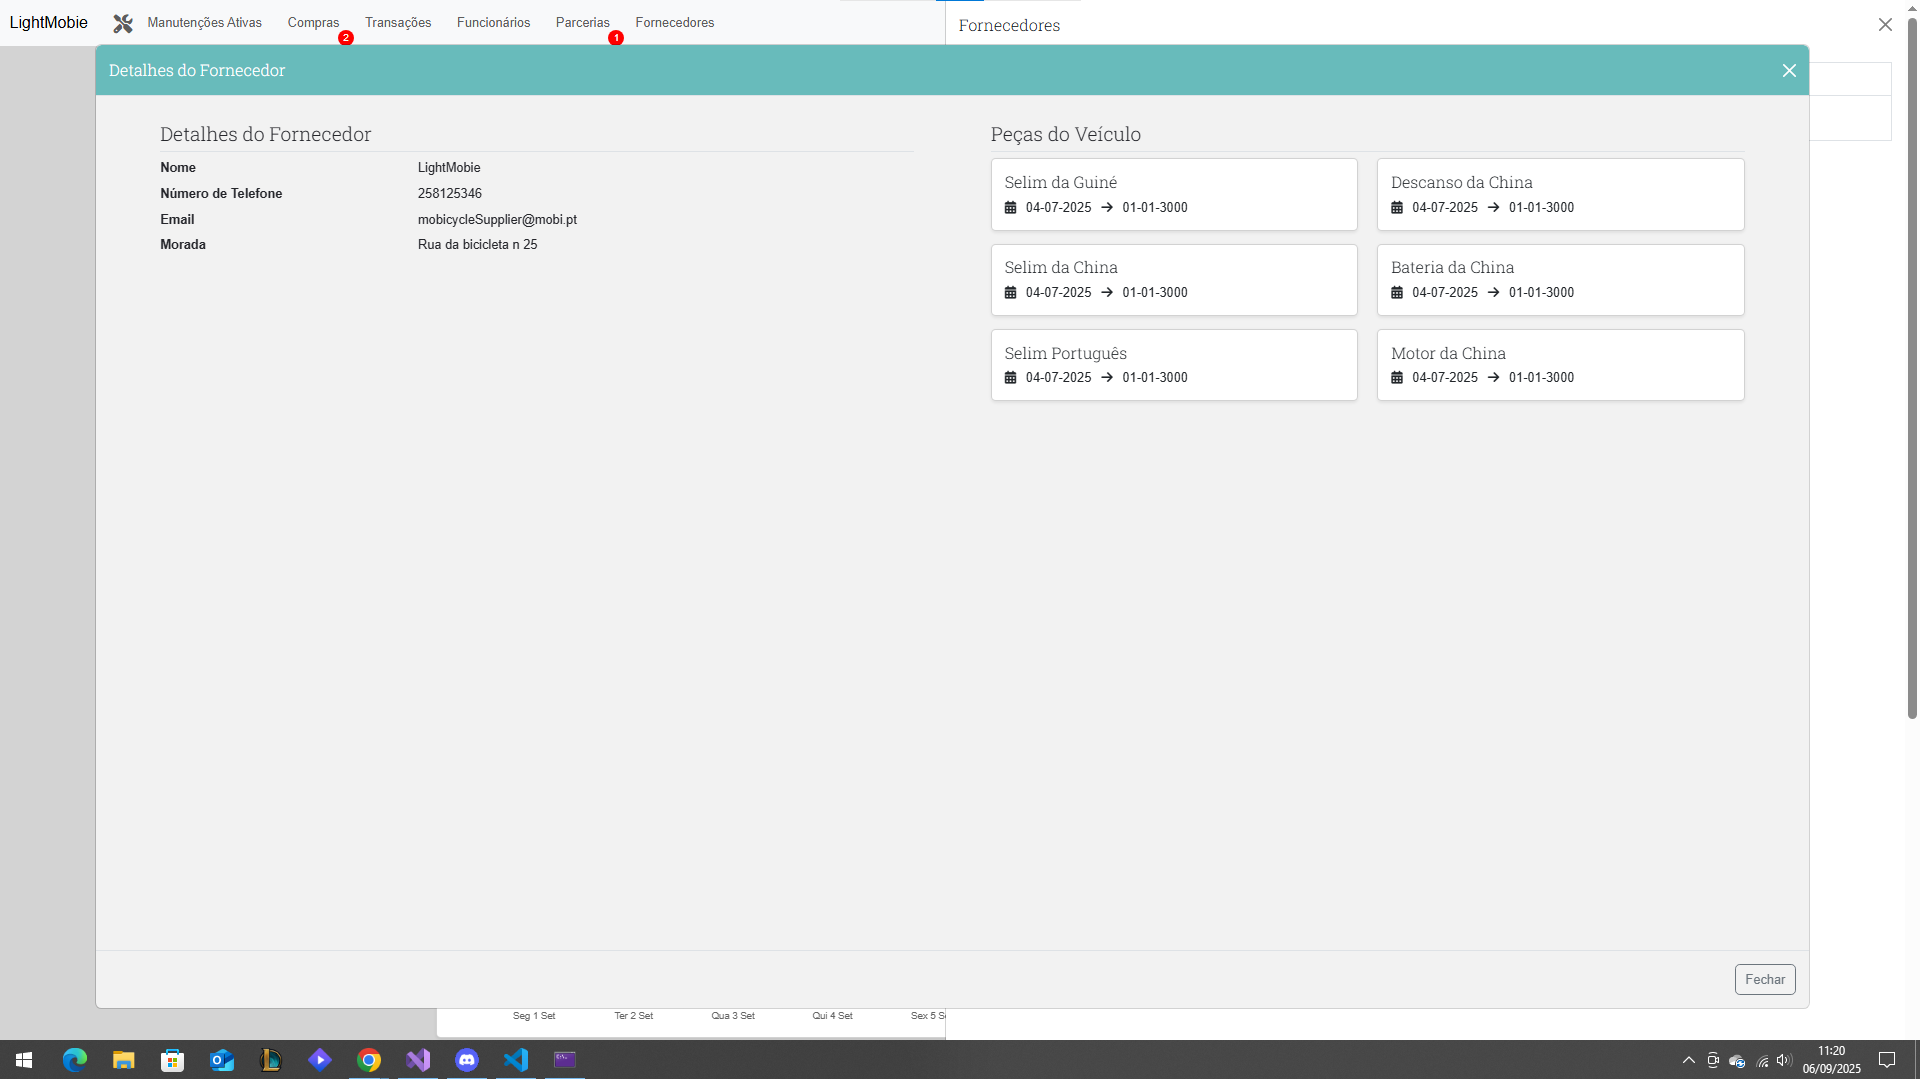
\includegraphics[width=\textwidth]{figs/Implementation/workshopmanager/supplierDetails}
  \label{fig:workshopmanagerupplierDetails}
\end{figure}




\begin{figure}[h]
  \caption{Task type edit.}
  \centering
  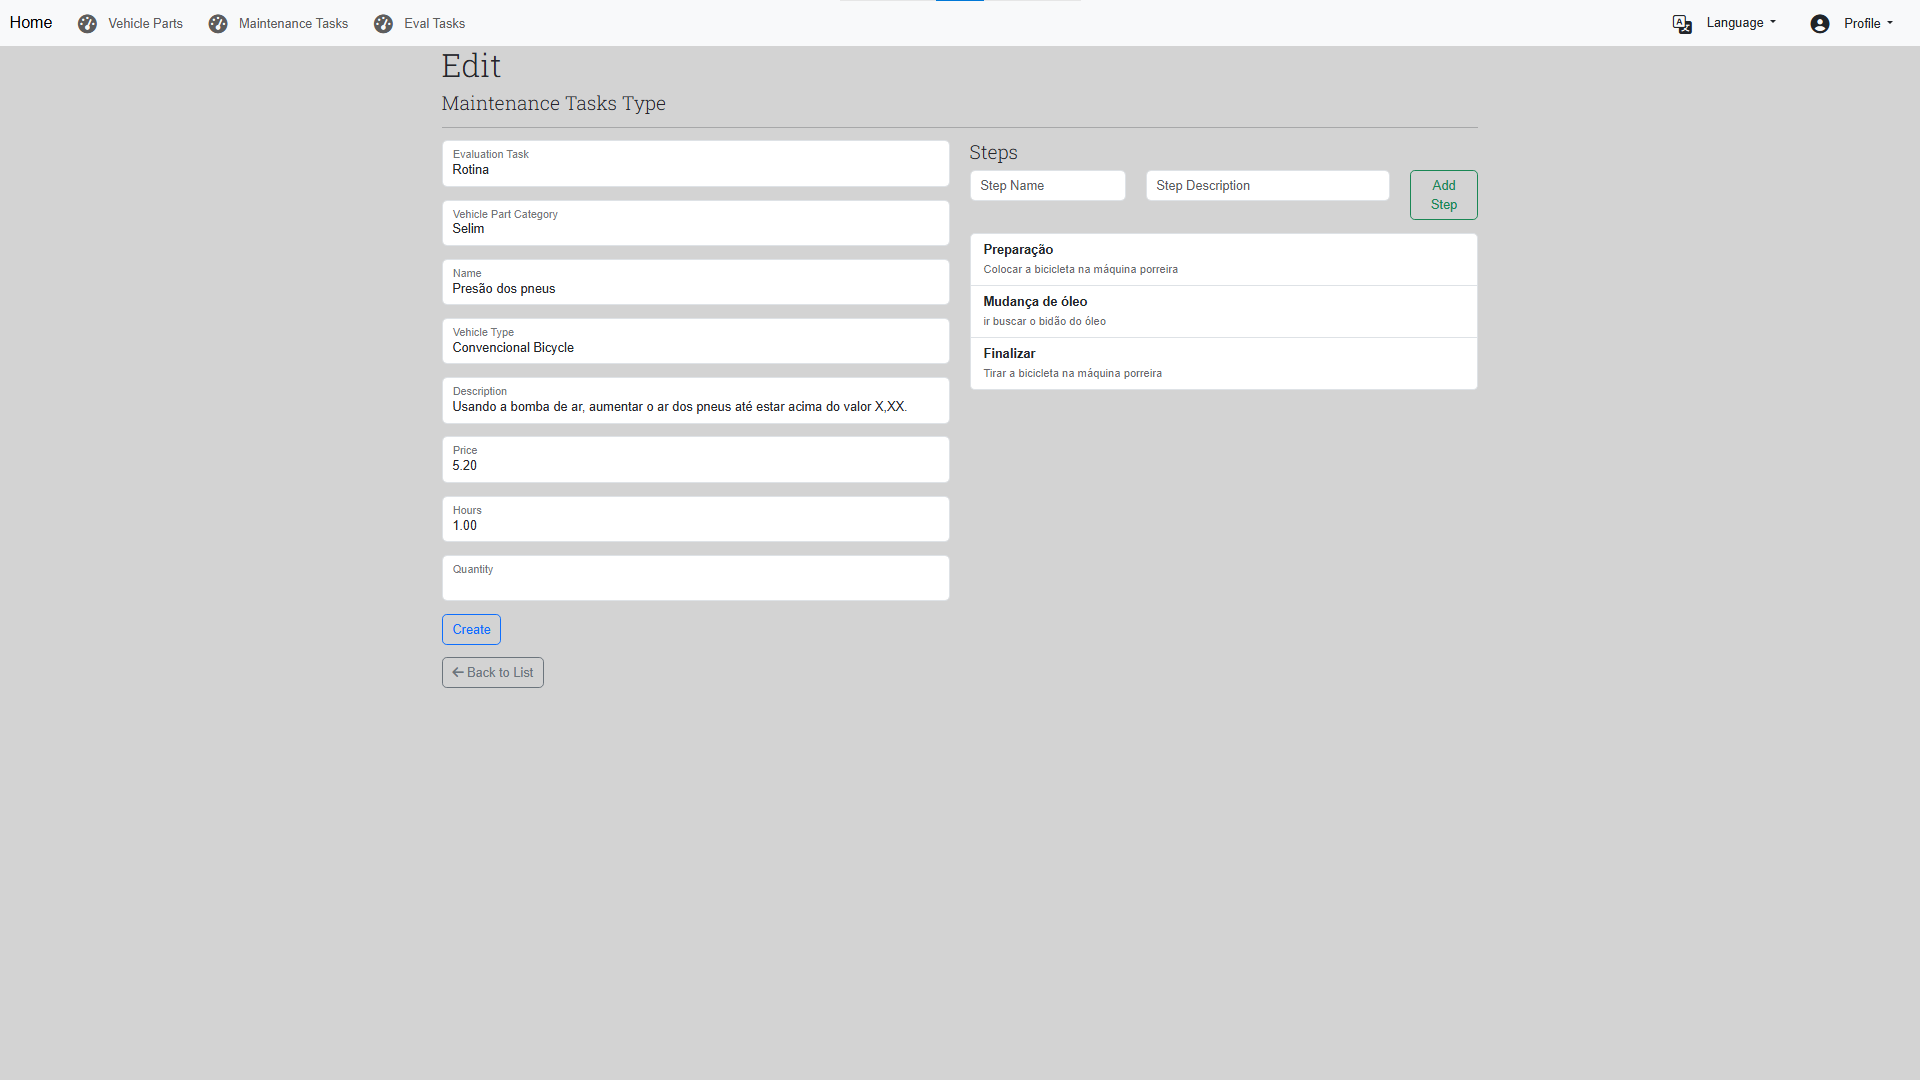
\includegraphics[width=\textwidth]{figs/Implementation/dealershipAdmin/taskEdit}
  \label{fig:taskEdit}
\end{figure}


\begin{figure}[h]
  \caption{Task type details.}
  \centering
  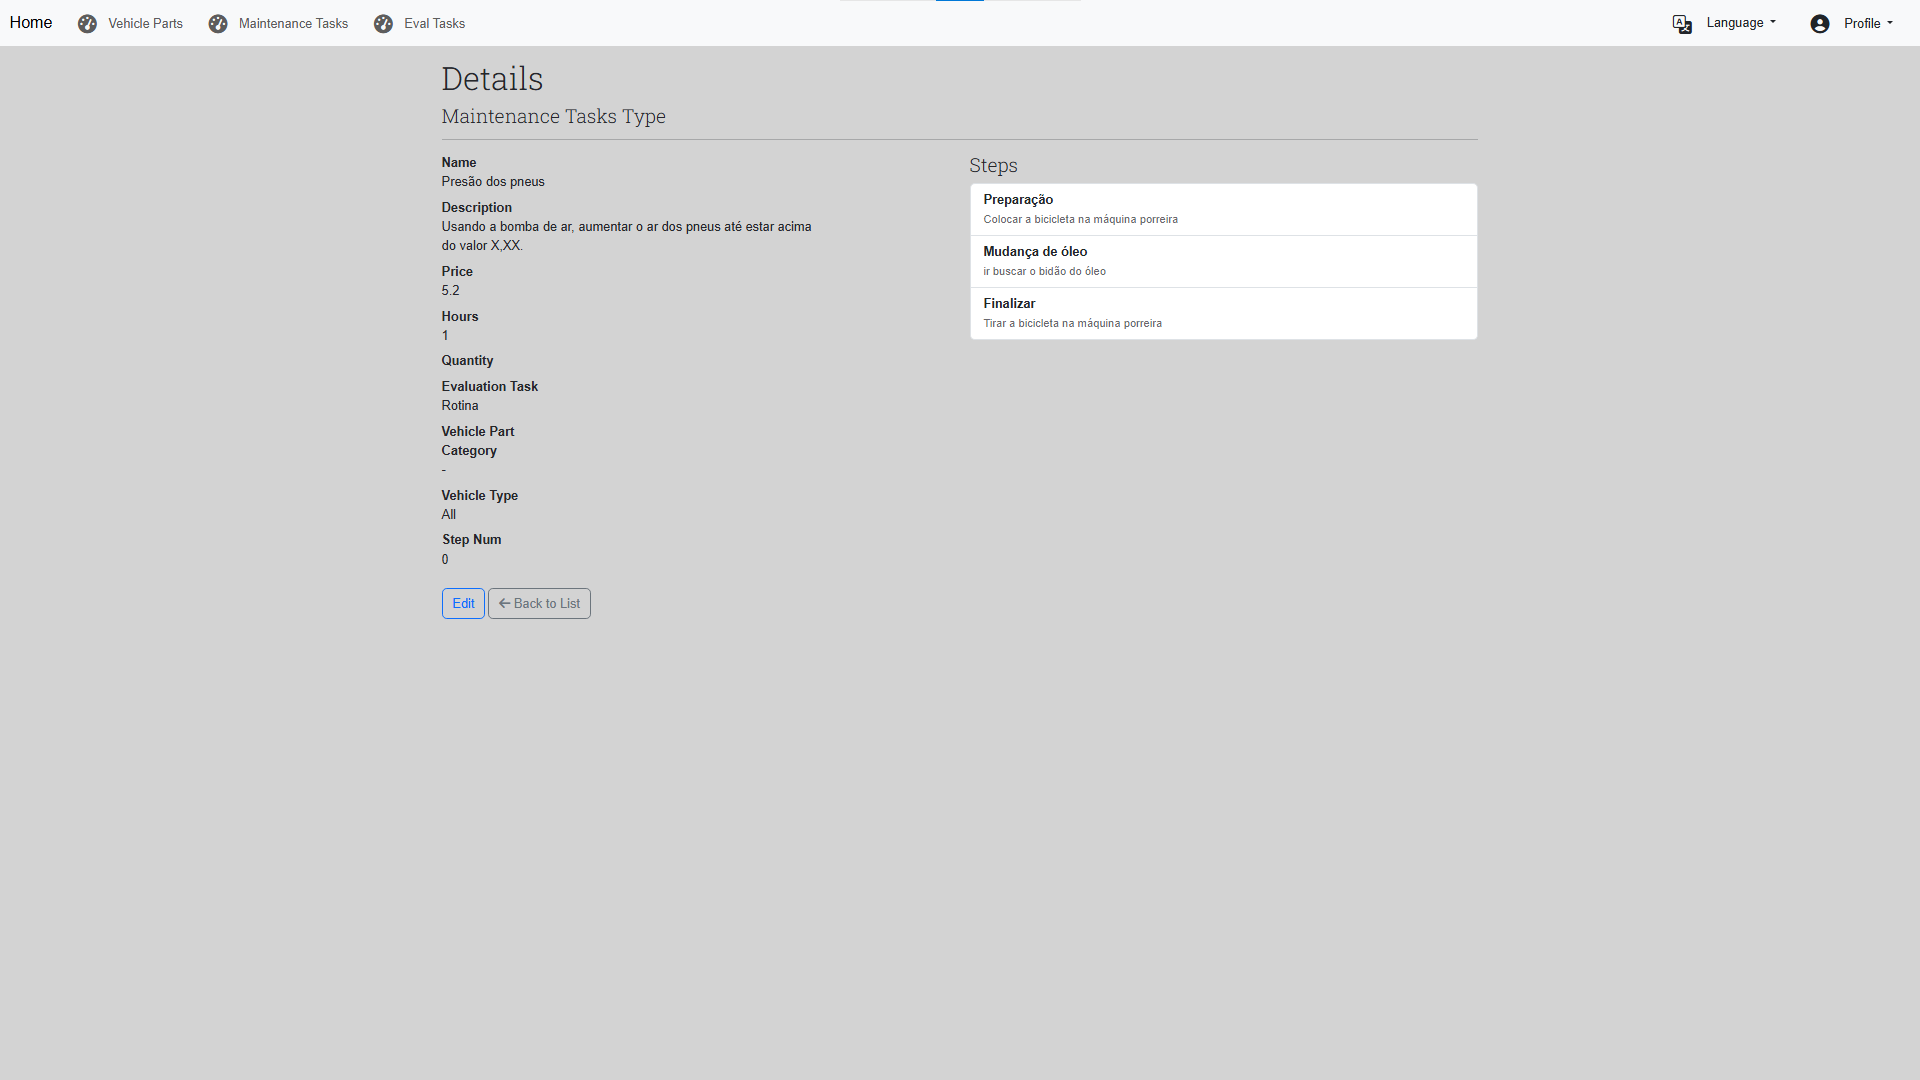
\includegraphics[width=\textwidth]{figs/Implementation/dealershipAdmin/taskDetails}
  \label{fig:taskDetails}
\end{figure}

 
\begin{figure}[h]
  \caption{Task type delete.}
  \centering
  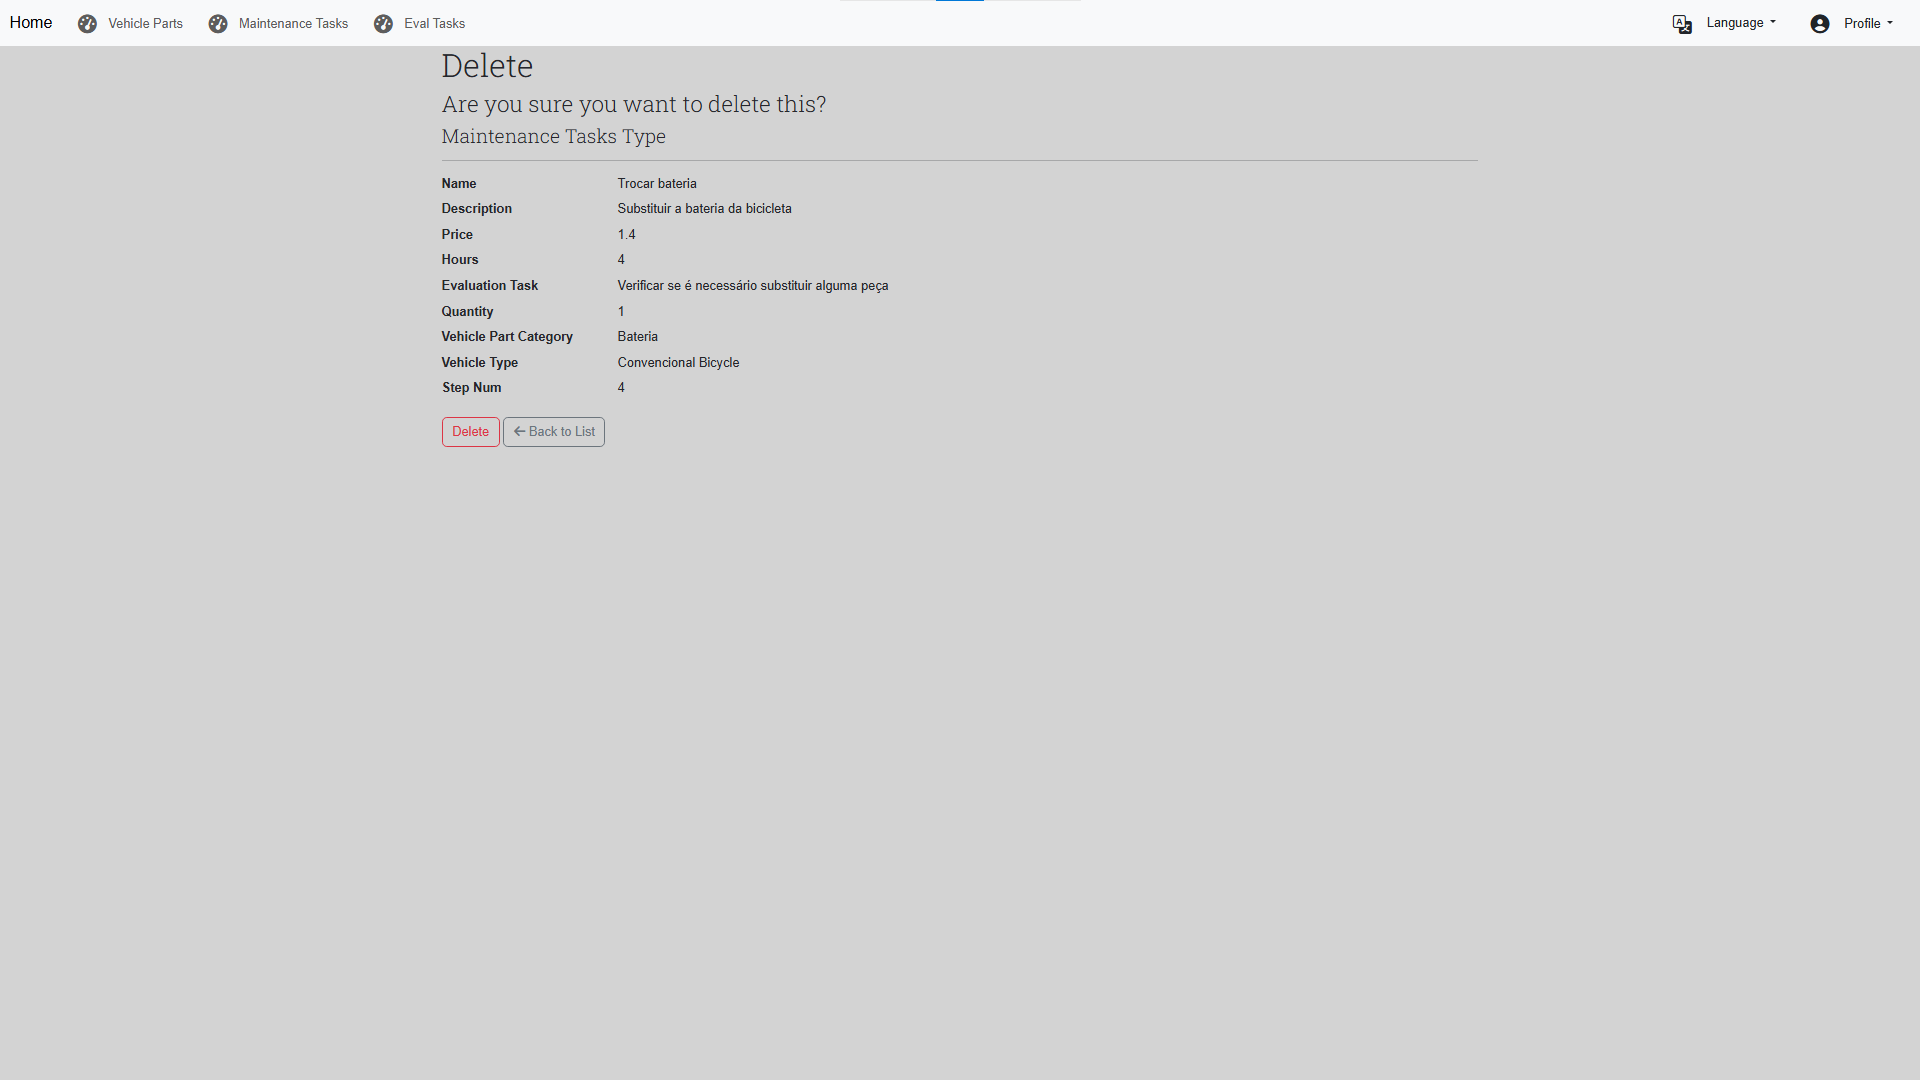
\includegraphics[width=\textwidth]{figs/Implementation/dealershipAdmin/taskDelete}
  \label{fig:taskDelete}
\end{figure}

\begin{figure}[h]
  \caption{Task type create.}
  \centering
  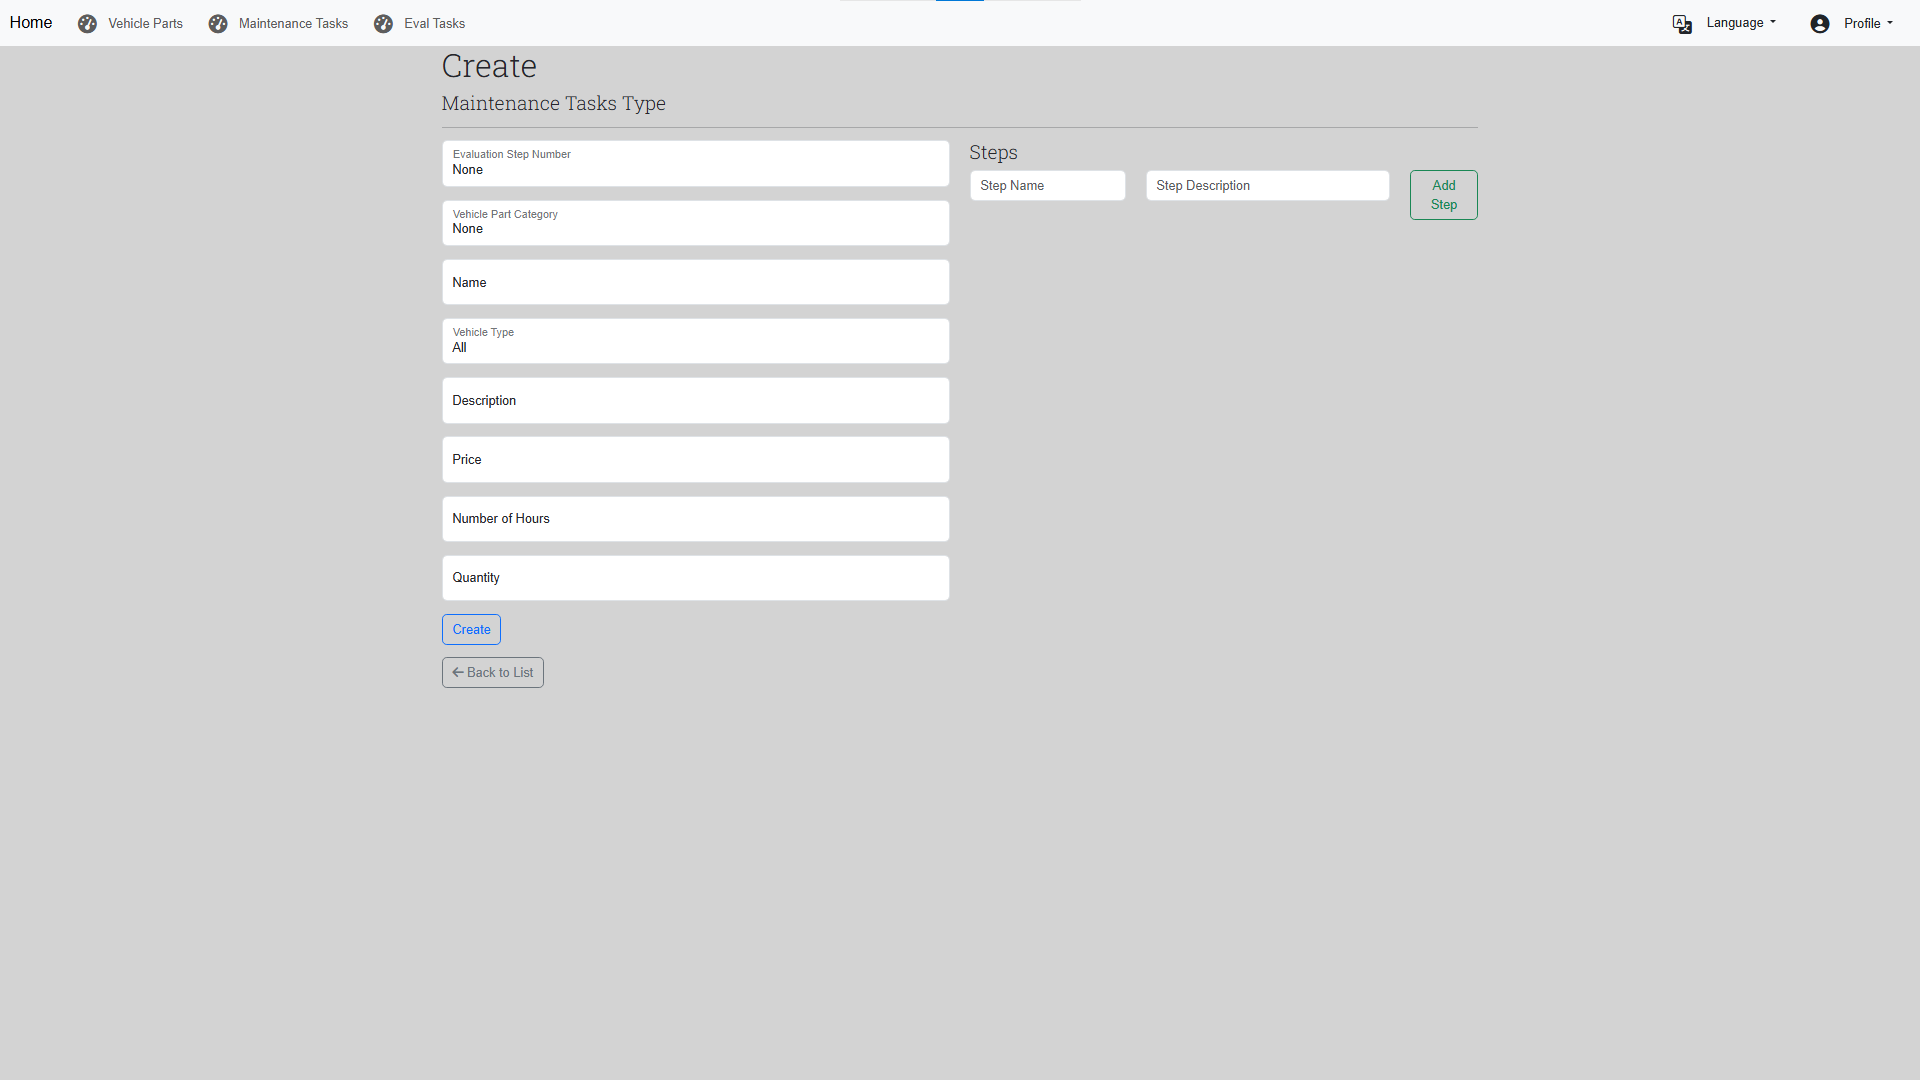
\includegraphics[width=\textwidth]{figs/Implementation/dealershipAdmin/taskCreate}
  \label{fig:taskCreate}
\end{figure}


\end{figure}
\begin{figure}[h]
  \caption{Eval task create.}
  \centering
  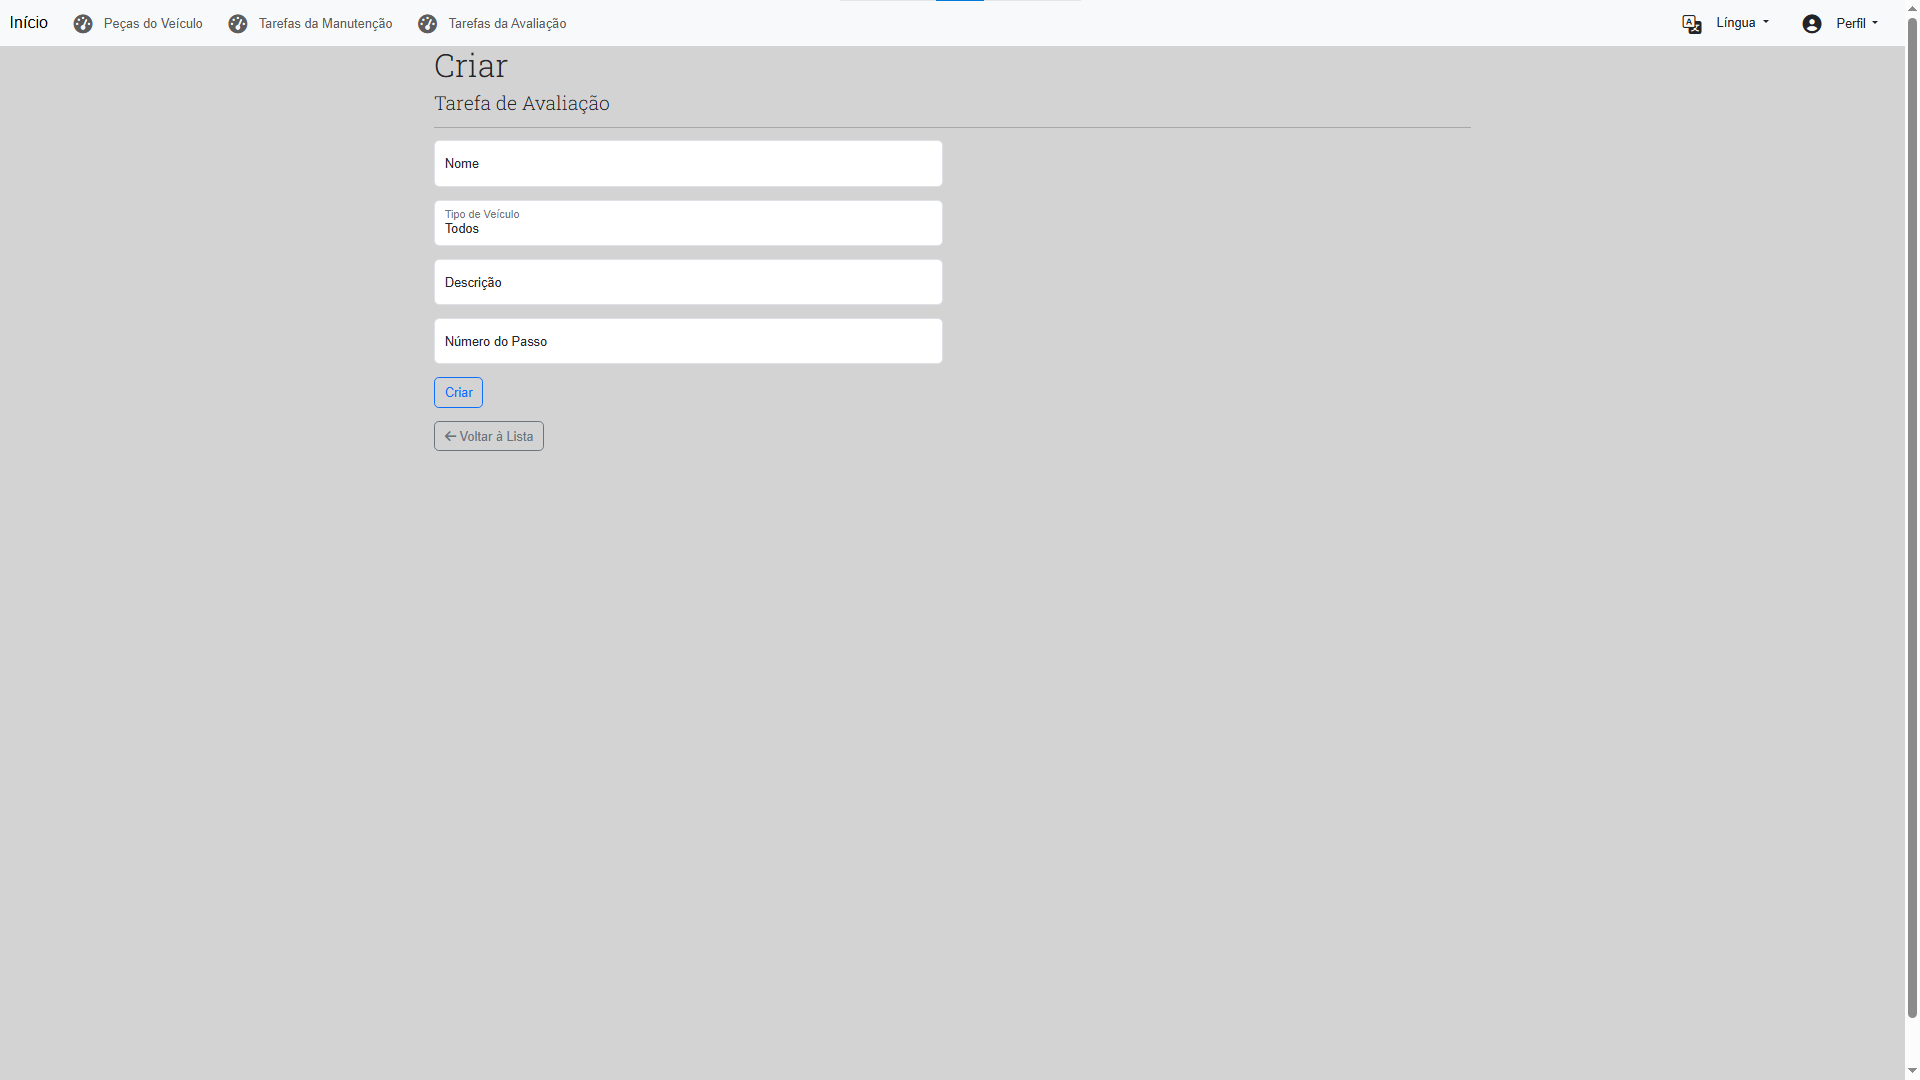
\includegraphics[width=\textwidth]{figs/Implementation/dealershipAdmin/evalCreate}
  \label{fig:evalCreate}
\end{figure}

\begin{figure}[h]
  \caption{Eval task delete.}
  \centering
  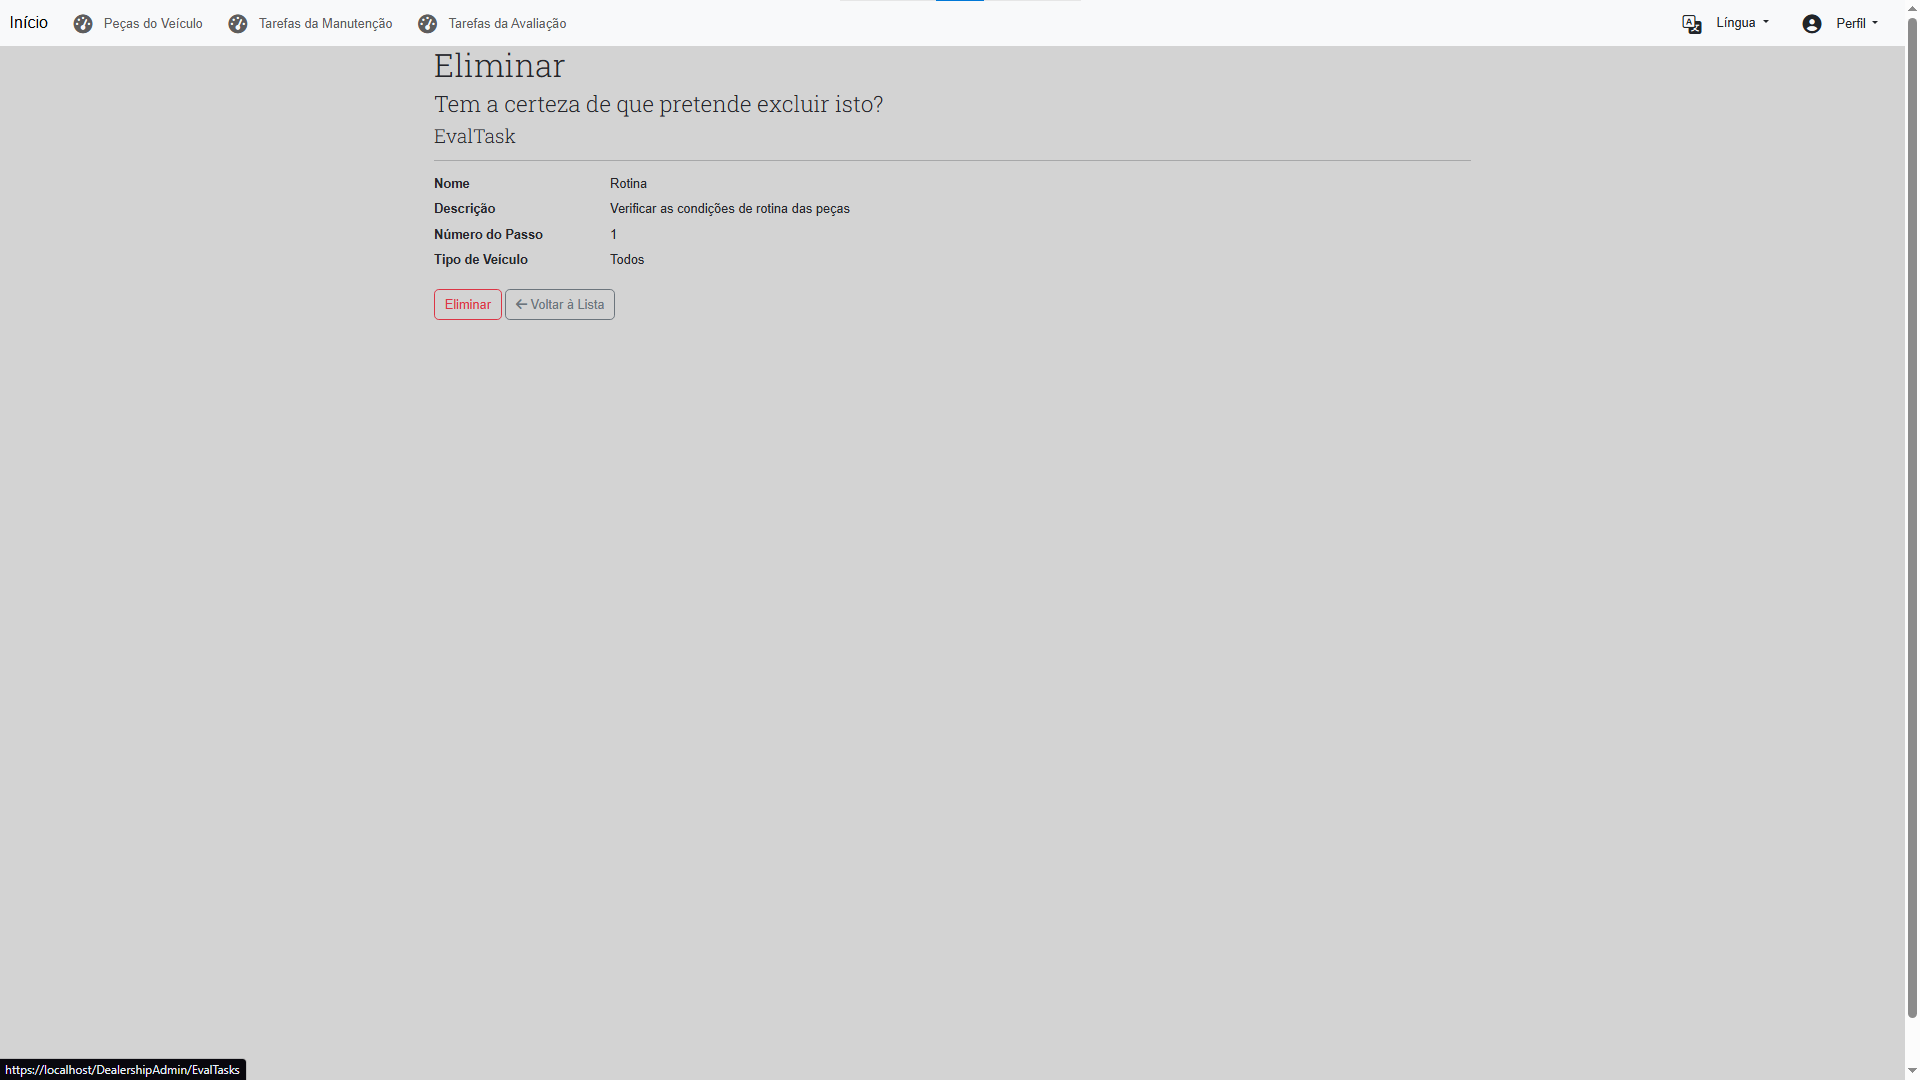
\includegraphics[width=\textwidth]{figs/Implementation/dealershipAdmin/evalDelete}
  \label{fig:evalDelete}
\end{figure}

\begin{figure}[h]
  \caption{Eval task details.}
  \centering
  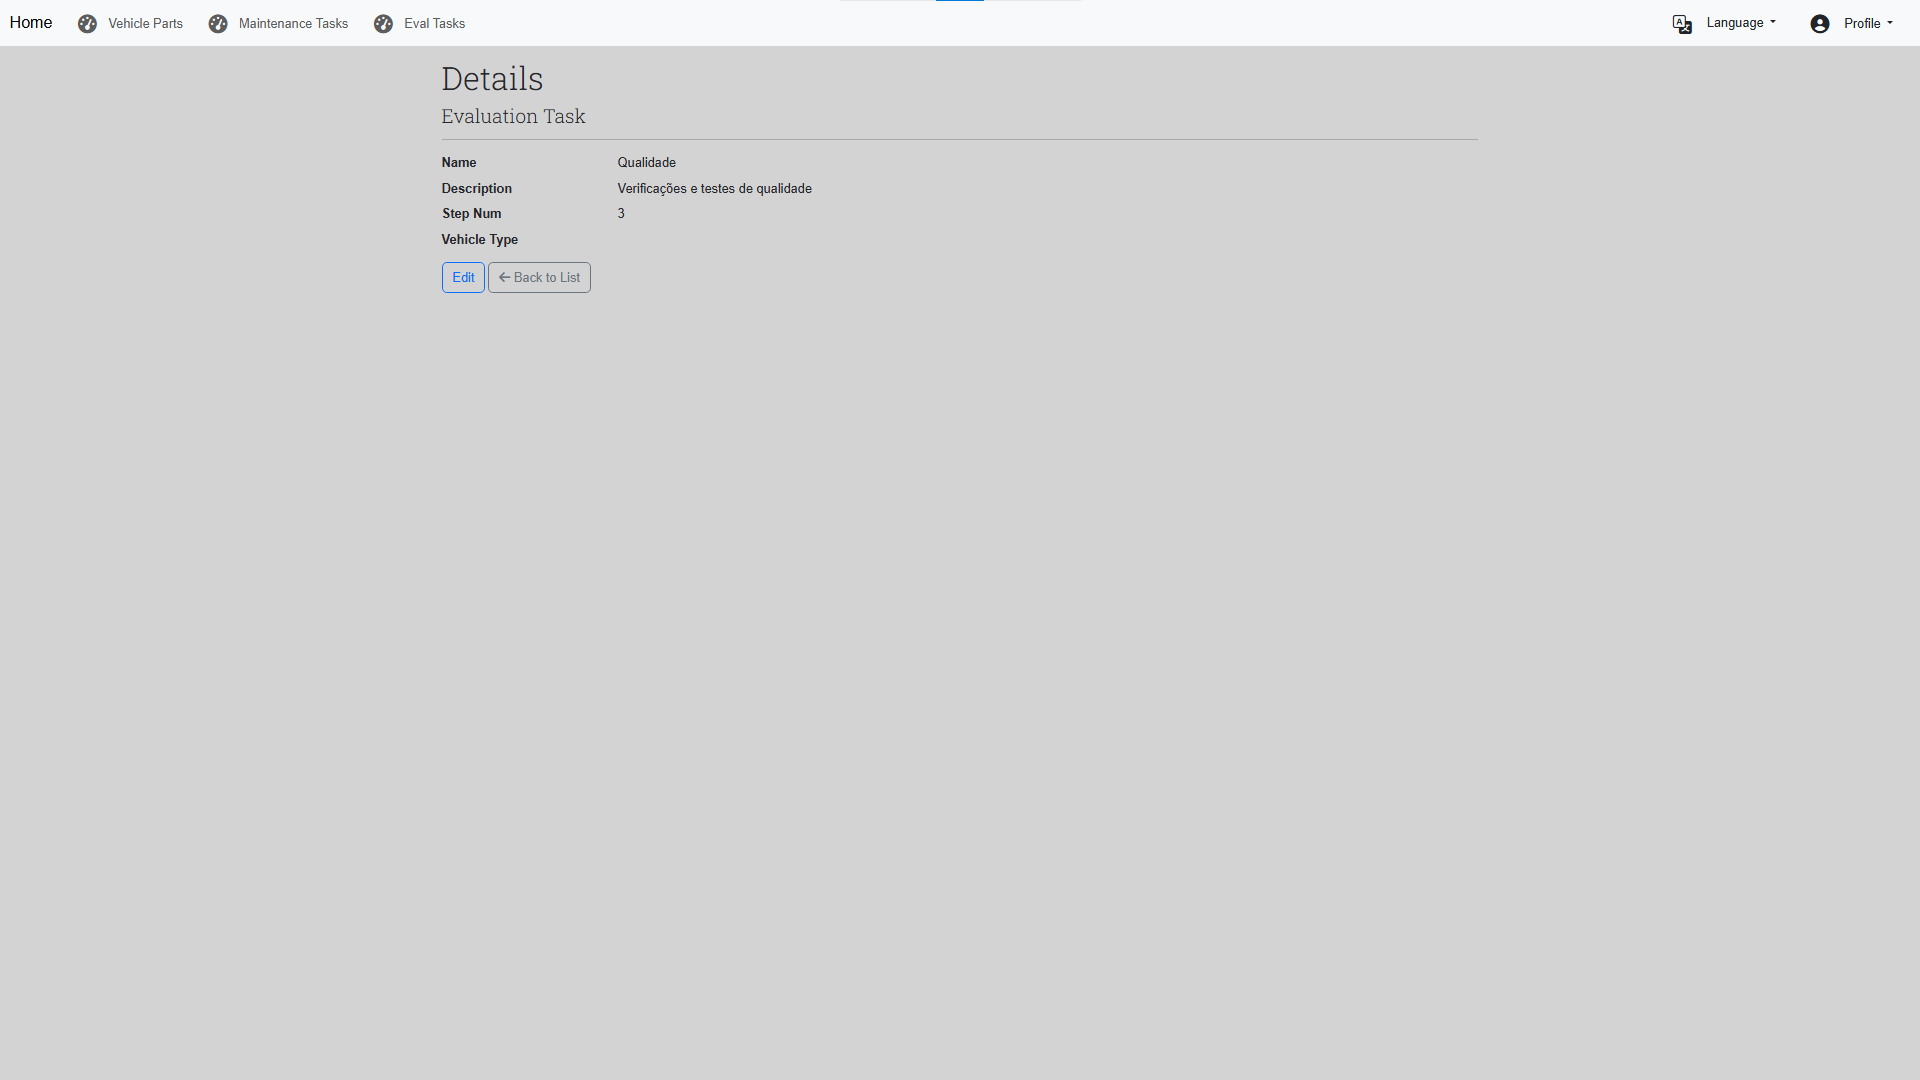
\includegraphics[width=\textwidth]{figs/Implementation/dealershipAdmin/evalDetails}
  \label{fig:evalDetails}
\end{figure}


\begin{figure}[h]
  \caption{User tests tasks}
  \centering
  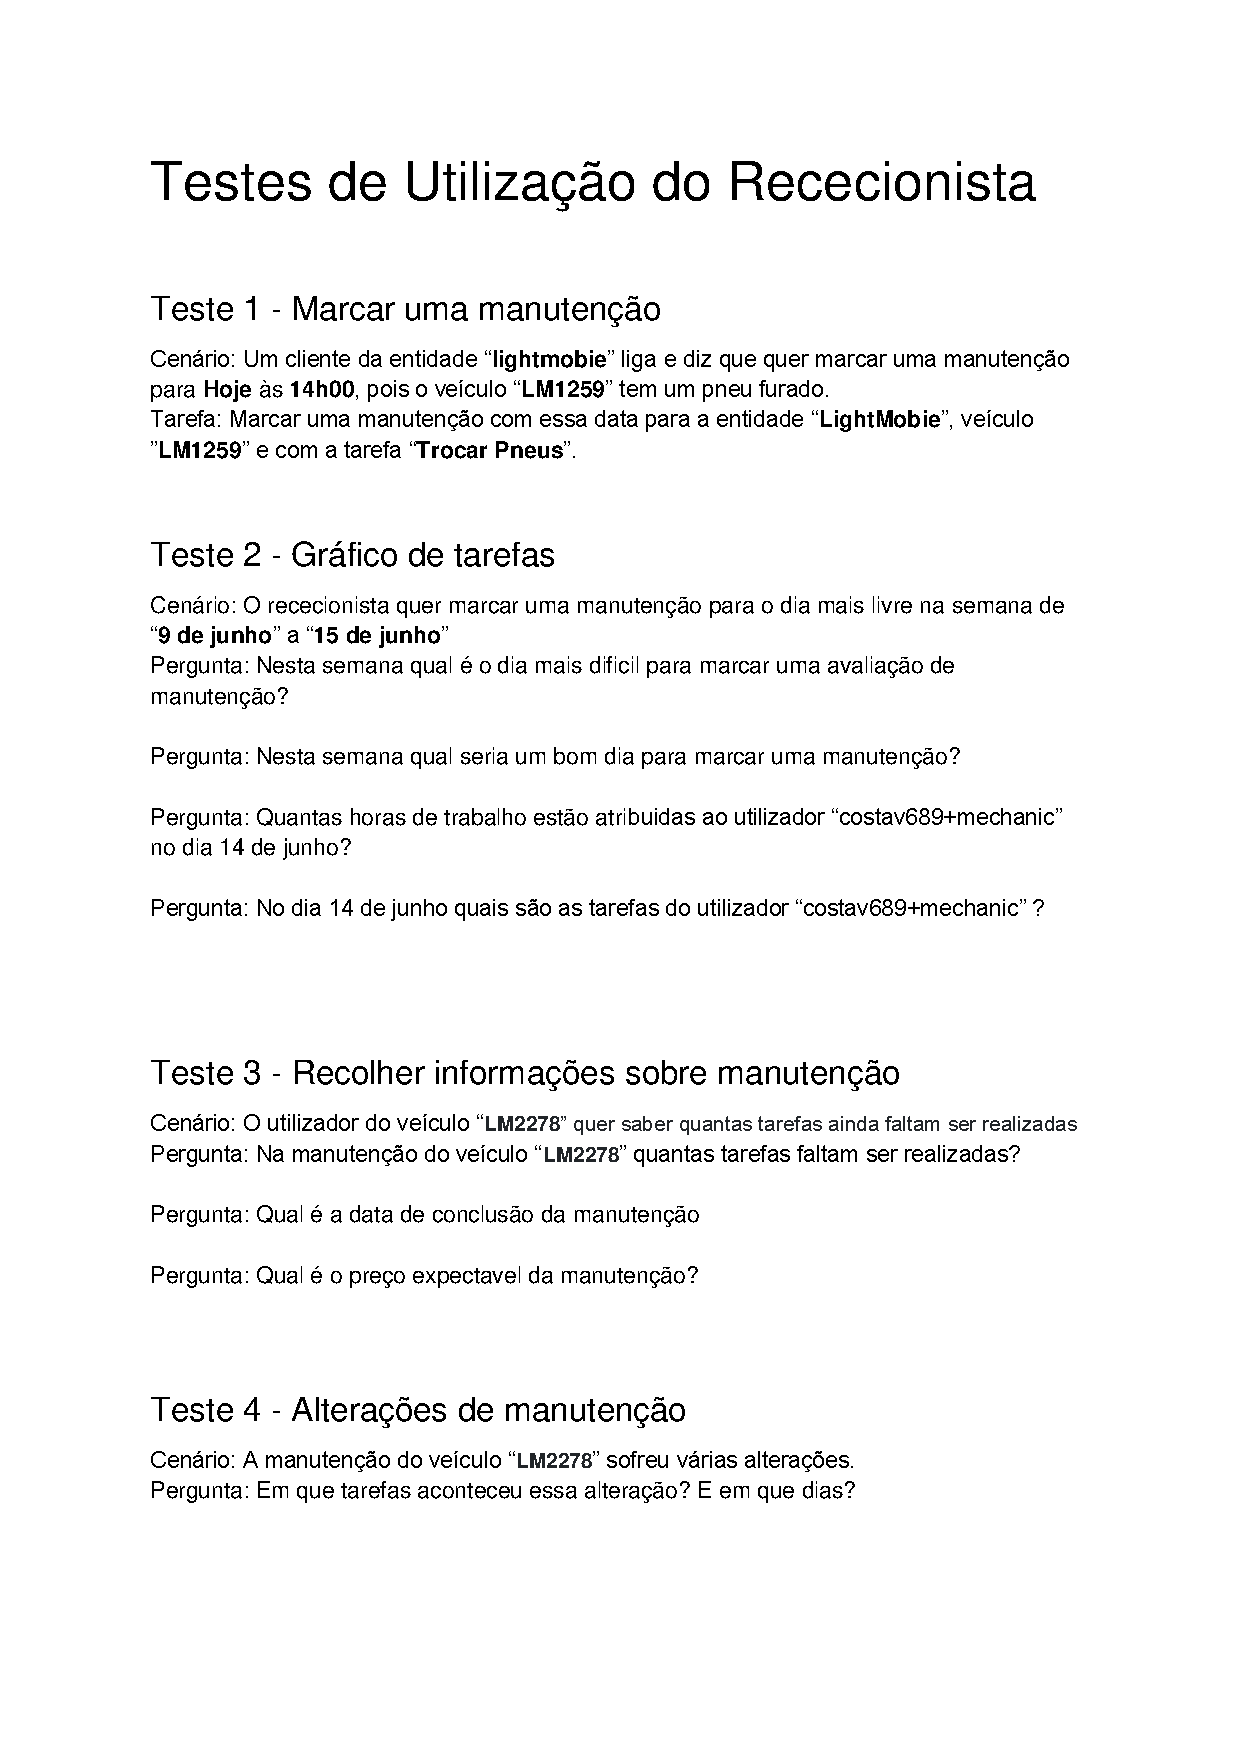
\includegraphics[width=0.75\textwidth]{figs/chapter5/UserTestsTasks}
  \label{fig:UserTestsTasks}
\end{figure}

\begin{figure}[h]
  \caption{Aplication questionaire}
  \centering
  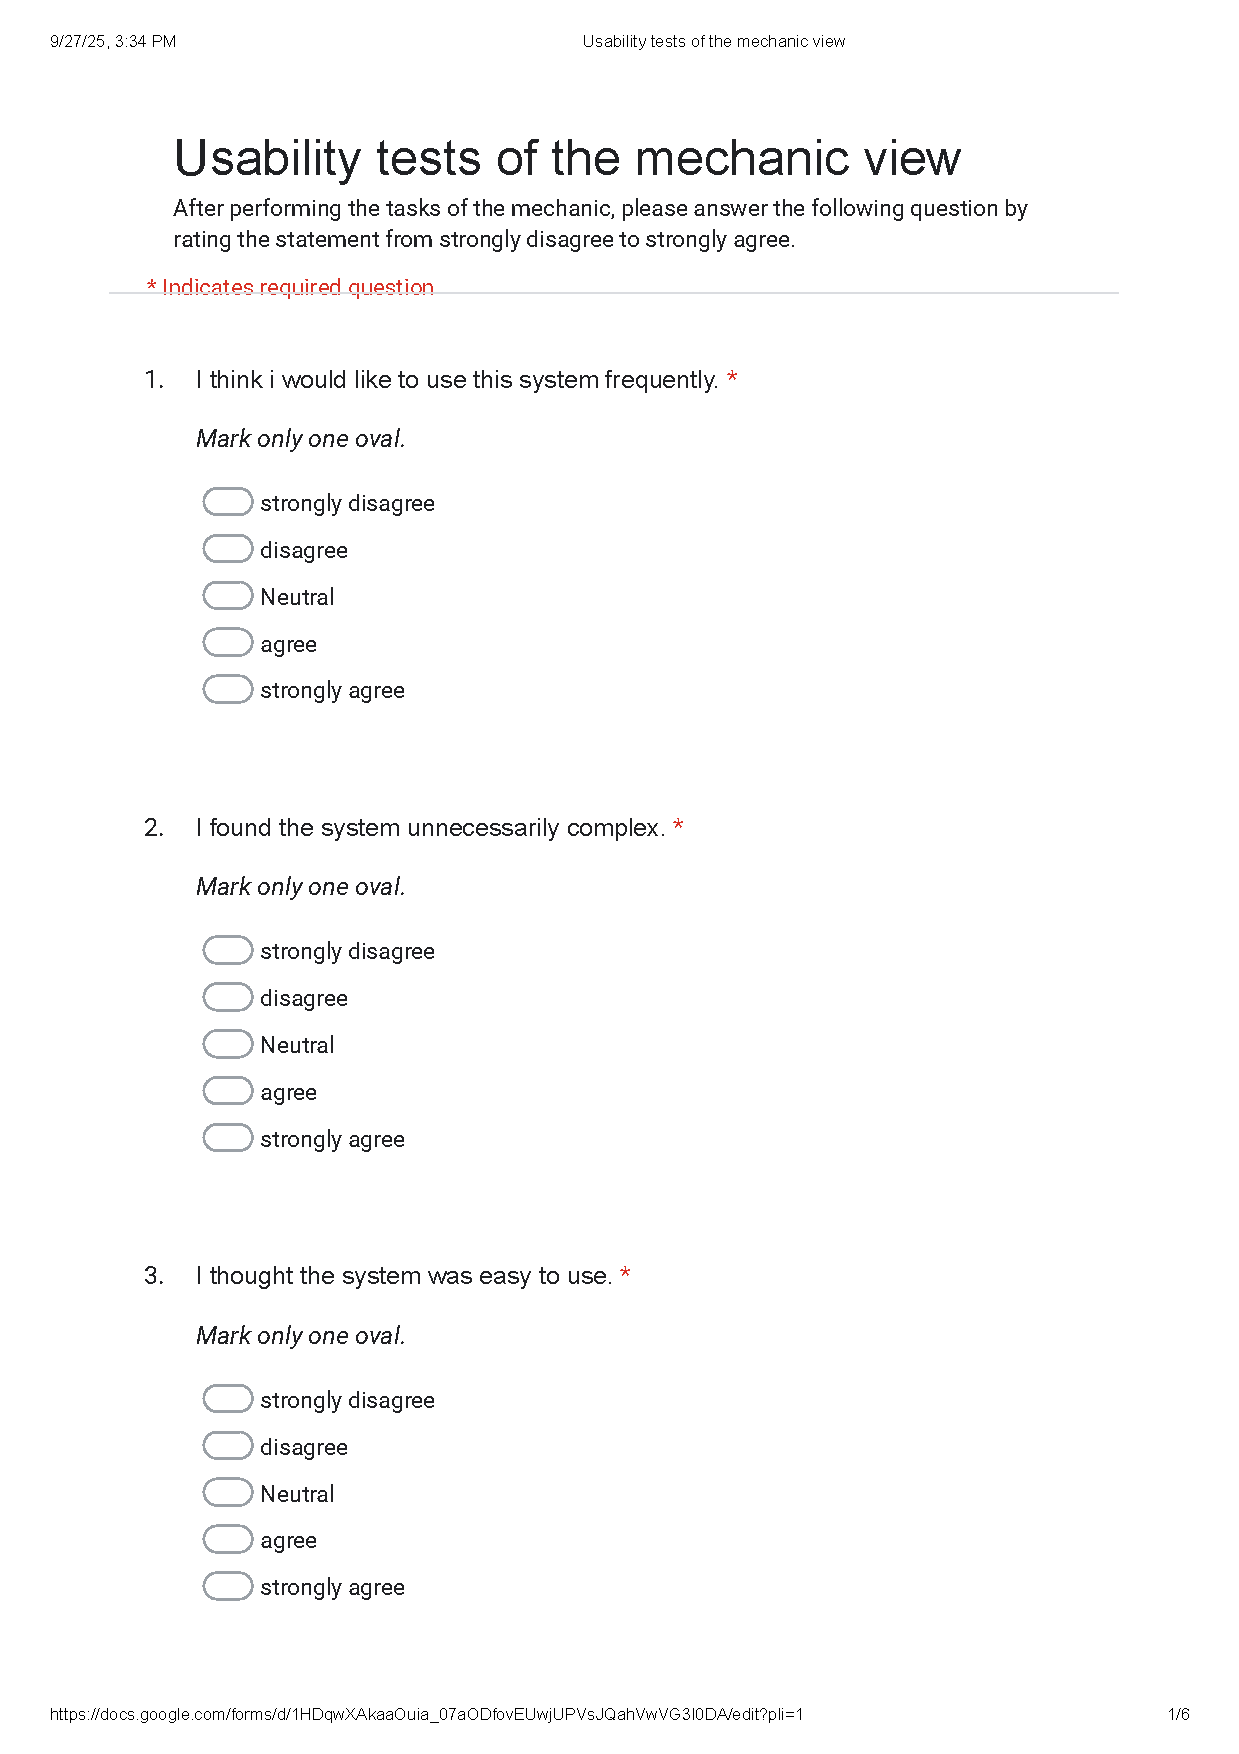
\includegraphics[width=0.75\textwidth]{figs/chapter5/AplicationQuestionaire}
  \label{fig:AplicationQuestionaire}
\end{figure}